\documentclass[11pt]{amsart}
\usepackage[T1]{fontenc}
\usepackage[utf8]{inputenc}
\usepackage{lmodern}
\usepackage[margin=1in]{geometry}
\usepackage{amsmath}
\usepackage{amssymb}
\usepackage{amsfonts}
\usepackage{amsthm}
\usepackage{mathtools}
\usepackage{booktabs,array,longtable}
\usepackage{microtype}
\usepackage{enumitem}
\usepackage{xcolor}
\usepackage{verbatim}
\usepackage{graphicx}
\usepackage{listings}
\numberwithin{equation}{section}
\setcounter{tocdepth}{3}
\setcounter{secnumdepth}{3}
\allowdisplaybreaks
\usepackage[hidelinks]{hyperref}
\graphicspath{{figures/}}
\lstset{
 basicstyle=\ttfamily\scriptsize,
 breaklines=true,
 breakatwhitespace=false,
 columns=fullflexible,
 keepspaces=true,
 showstringspaces=false
}

\newtheorem{theorem}{Theorem}[section]
\newtheorem{proposition}[theorem]{Proposition}
\newtheorem{lemma}[theorem]{Lemma}
\newtheorem{corollary}[theorem]{Corollary}
\newtheorem{hypothesis}[theorem]{Hypothesis}
\theoremstyle{definition}
\newtheorem{definition}[theorem]{Definition}
\newtheorem{experiment}[theorem]{Experiment}
\newtheorem{heuristic}[theorem]{Heuristic}
\theoremstyle{remark}
\newtheorem{remark}[theorem]{Remark}
\newtheorem{warning}[theorem]{Warning}

\newcommand{\RH}{\mathrm{RH}}
\newcommand{\dd}{\,\mathrm d}
\newcommand{\CN}{C_N}
\newcommand{\SN}{S_N}
\newcommand{\Log}{\operatorname{Log}}
\newcommand{\Ree}{\operatorname{Re}}
\newcommand{\Imm}{\operatorname{Im}}
\newcommand{\cP}{\mathcal P}
\newcommand{\cB}{\mathcal B}

\title[Triangular centroids of zeta ordinates]{Triangular Centroids of Exponential Walks on Riemann Zeta Ordinates\\
and the Riemann--von Mangoldt Clock\\[0.4em]
\large Unconditional linearization, a smooth-clock limit, and a centroid-family equivalence to RH}
\author{Víctor Casaña-Giner}
\thanks{Bio Logic Crop Science S.L., E-46120 Alboraya (Valencia), Spain. E-mail: \texttt{vcasana@biologiccropscience.com}. ORCID: 0000-0002-8252-2608.}
\date{August 2026}

\begin{document}

\begin{abstract}
Let $0<\gamma_1\leq\gamma_2\leq\cdots$ be the positive ordinates of the nontrivial zeros of the Riemann zeta function and let
\begin{equation}\label{eq:abstract_centroid}
C_N^{\zeta}=\frac1N\sum_{k\leq N}(N-k+1)e^{i\gamma_k}.
\end{equation}
The sequence $\gamma_k$ enumerates every upper-half-plane zero individually with algebraic multiplicity; equal positive ordinates are therefore repeated. We separate this ordinal triangular centroid from the centroid of the synthetic Riemann--von Mangoldt clock. With the exact Riemann--Siegel counting clock $H(x)=1+\vartheta(x)/\pi$ and the midpoint argument term $S_*(\gamma)=\mathcal N_*(\gamma)-H(\gamma)$ at a distinct positive ordinate $\gamma$, an unconditional Stieltjes decomposition gives
\begin{equation}\label{eq:abstract_level1_short}
C_N^{\zeta}-Q_N^{(H)}\longrightarrow0.
\end{equation}
The same reduction proves that the true-zero Landau-weighted statistic
\begin{equation}\label{eq:abstract_true_zero_landau}
L_N^{(M)}=\sum_{k\leq N}\left(1-\frac{M(\gamma_k)}{M(\gamma_N)}\right)e^{i\gamma_k}
\end{equation}
has the same asymptotic target: $L_N^{(M)}-C_N^{\zeta}\to0$ unconditionally. This does not replace $\gamma_k$ by the Lambert inverse levels $\tau_k$.

For the synthetic clock $M(\tau_k)=k-\tfrac12$, the inverse is explicit through Lambert $W$; its exponential centroid is proved to converge and is represented by a conditionally convergent Abel series. For the true zeta centroid, the symmetric explicit formula at logarithmic frequency $u=1$ yields, under RH and a stated Riesz-compatibility hypothesis,
\begin{equation}\label{eq:abstract_real_constant_short}
\Re C_\infty^{\zeta}=\frac{1}{2\sqrt e}\left(e-\frac1{e^2-1}\right),
\end{equation}
and a separate one-sided boundary-interchange hypothesis gives the conditional complex value
\begin{equation}\label{eq:abstract_complex_constant_short}
C_\infty^{\zeta}=0.77689426079325\ldots+0.76785566886455\ldots i.
\end{equation}
The same ordinal centroid extends to the complex-frequency family $C_N^{\zeta}(u)$. For $\Im u>0$ both the ordinate centroid and a completed-zero companion have absolutely convergent holomorphic limits. On the positive imaginary axis their difference is a positive Laplace sum, and its vanishing at any one fixed $iy$, $0<y\le4\pi$, is equivalent to RH. The criterion is therefore obtained from the centroid family itself. The experimentally observed point $u=1$ is a distinct real-boundary statistic and is not identified with the interior completed-zero series.
\end{abstract}

\maketitle

\noindent\textbf{Keywords.} Riemann zeta function; zero ordinates; exponential sums; triangular centroid; Cesàro summation; Riesz means; Riemann--von Mangoldt formula; Lambert $W$; Riemann--Siegel theta function; explicit formula; Selberg second moment; Landau--Gonek formula; Fujii horizontal moment; Riemann hypothesis.

\medskip
\noindent\textbf{MSC 2020.} 11M06; 11M26; 11M36; 11Y35.


\tableofcontents
\newpage

\section*{List of notation}\label{sec:notation}
The recurring symbols are fixed as follows. Dummy variables used only inside a single integral or finite sum are not listed.
\begin{longtable}{@{}p{0.22\textwidth}p{0.72\textwidth}@{}}
\toprule
Symbol & Meaning \\
\midrule
\endfirsthead
\toprule
Symbol & Meaning \\
\midrule
\endhead
$k=1,2,\ldots,N$ & Ordinal zero index. Distinct indices may have the same ordinate. \\
$N$ & Final value of the ordinal index $k$ in a finite truncation; it is not a second running index. \\
$\rho_k=\beta_k+i\gamma_k$ & Nontrivial zeros of $\zeta$, with $\gamma_k>0$, ordered by nondecreasing ordinate and counted with multiplicity. \\
$\nu(\gamma)$ & Total upper-half-plane multiplicity at a positive ordinate $\gamma$; it is the jump size of $\mathcal N$ there. \\
$\delta_\rho=\beta-\tfrac12$ & Horizontal displacement of a nontrivial zero from the critical line. The symbol $\delta$ is reserved for this horizontal displacement throughout the analytic part of the paper. \\
$\mathcal N(x)$ & Number of upper-half-plane nontrivial zeros with $0<\gamma\le x$, each zero counted with algebraic multiplicity. \\
$\mathcal N_*(\gamma)$ & Midpoint of the jump of $\mathcal N$ at a positive ordinate $\gamma$. \\
$\vartheta(x)$ & Riemann--Siegel theta function. \\
$H(x)=1+\vartheta(x)/\pi$ & Exact smooth Riemann--Siegel counting clock. \\
$S(x)$, $S_*(\gamma)$ & Classical argument term in $\mathcal N(x)=H(x)+S(x)$ away from zero ordinates and its midpoint value at a zero ordinate $\gamma$. \\
$r_k$ & Ordinal rank defect $r_k=k-\tfrac12-H(\gamma_k)$; this is the quantity entering the exact finite centroid identity. \\
$r_k^{(M)}$ & Main-clock ordinal defect $k-\tfrac12-M(\gamma_k)$. \\
$M(x)$ & Principal smooth Riemann--von Mangoldt clock $\frac{x}{2\pi}\log\frac{x}{2\pi e}+\frac78$. \\
$\tau_k$ & Lambert inverse level defined by $M(\tau_k)=k-\tfrac12$. \\
$\varepsilon_k=\gamma_k-\tau_k$ & Vertical zero--RVM discrepancy; this symbol is kept distinct from $\delta_\rho=\beta-\tfrac12$. \\
$b_k=e^{i\gamma_k}-e^{i\tau_k}$ & Paired phase residual obtained by subtracting after exponentiation. \\
$a_k=e^{i\varepsilon_k}-1$ & Centered intrinsic residual obtained by subtracting the ordinates first and then exponentiating. \\
$R_k^{\mathrm{RVM}}$, $A_k^{\mathrm{RVM}}$ & Running partial sums $\sum_{j\le k}b_j$ and $\sum_{j\le k}a_j$, $k=1,\ldots,N$. \\
$\mathcal R_{\mathrm{RVM}}(y)$, $\mathcal A_{\mathrm{RVM}}(y)$ & Damped zero--RVM residual and its completed-zero comparison in Corollary~\ref{cor:RVM_residual_RH_equivalence}. \\
$\widehat\tau_k$ & Exact smooth level defined by $H(\widehat\tau_k)=k-\tfrac12$. \\
$g_k$ & Smooth-clock gap $g_k=\tau_{k+1}-\tau_k$. \\
$v_k$ & Smooth-clock phase $v_k=e^{i\tau_k}$. \\
$d_k$, $q_k$ & Abel coefficients for the synthetic Lambert walk: $d_k=(e^{ig_k}-1)^{-1}$ and $q_k=d_{k+1}-d_k$. \\
$S_N^{\zeta}$ & Zeta exponential walk $\sum_{k\le N}e^{i\gamma_k}$. \\
$C_N^{\zeta}$ & Original triangular centroid at real frequency $u=1$. \\
$w_{k,N}$ & Triangular weight $1-(k-1)/N$. \\
$Q_N^{(H)}$, $Q_N^{(M)}$ & Linearized true-zero statistics using the exact clock $H$ or the main clock $M$. \\
$L_N^{(M)}$ & True-zero Landau-weighted statistic; the ordinates remain the actual $\gamma_k$. \\
$M_N^{\mathrm{end}}$ & Endpoint clock value $M(\gamma_N)$ used in the proof of the true-zero weighted target. \\
$S_N^M$, $C_N^M$ & Exponential walk and triangular centroid of the synthetic Lambert levels $\tau_k$. \\
$C_N^{\zeta}(u)$ & Complex-frequency extension of the original ordinal centroid; $C_N^{\zeta}(1)=C_N^{\zeta}$. \\
$C^{\zeta}(u)$ & Holomorphic interior limit of $C_N^{\zeta}(u)$ for $\Im u>0$. \\
$C_N^{\xi}(u)$ & Finite completed-zero centroid using the same triangular weights and the factors $e^{u(\rho_k-1/2)}$. \\
$C^{\xi}(u)$ & Holomorphic interior limit of $C_N^{\xi}(u)$ for $\Im u>0$. \\
$\mathcal D(y)$ & Positive imaginary-axis defect $C^{\zeta}(iy)-C^{\xi}(iy)$, $y>0$. \\
$\cB(x_0)$, $\cP_{\infty,\sigma}(x_0)$ & Smooth and arithmetic pieces of the one-sided boundary transform, with auxiliary height cutoff $x_0<\gamma_1$. \\
$C_\infty^{\zeta}$ & Conditional ordinal-centroid limit under RH and the stated boundary-interchange hypothesis; it is distinct from the interior series $C^{\xi}(u)$. \\
$A_2(x)$ & Fujii horizontal second-moment counting function with auxiliary height cutoff $x$. \\
$H_2(s)$, $F_2(z)$ & Dirichlet and Laplace transforms of the horizontal second-moment mass. \\
$\RH$ & Riemann hypothesis. \\
\bottomrule
\end{longtable}

\section{Introduction}\label{sec:introduction}

The present work grew from a simple numerical observation. I considered the exponential walk obtained by placing the positive ordinates of the nontrivial zeros of the Riemann zeta function on the unit circle and successively adding the corresponding vectors, and then compared its trajectory centroid with the centroid obtained when the same ordinal indices are replaced by a Lambert inversion of the smooth Riemann--von Mangoldt clock. The two constructions use almost indistinguishable ordinates at large height, but their centroids are strikingly different. This was the starting point of the paper: to understand what produces that difference, what part comes from the smooth counting law, what part belongs to the actual zeros, and how the centroid changes when the true-zero sequence is replaced by its smooth ordinal counterpart.

Write
\[
0<\gamma_1\leq\gamma_2\leq\cdots
\]
for the positive ordinates, counted with multiplicity, and let $\tau_k$ denote the paired Lambert--RVM levels defined by
\begin{equation}\label{eq:intro_rvm_levels}
M(\tau_k)=k-\frac12,
\qquad
M(x)=\frac{x}{2\pi}\log\frac{x}{2\pi e}+\frac78.
\end{equation}
At frequency one define
\begin{equation}\label{eq:intro_zeta_walk}
S_k^{\zeta}=\sum_{j=1}^{k}e^{i\gamma_j},
\qquad
S_k^{\mathrm{RVM}}=\sum_{j=1}^{k}e^{i\tau_j},
\qquad k=1,\ldots,N,
\end{equation}
and their triangular trajectory centroids by
\begin{equation}\label{eq:intro_centroid_definition}
C_N^{\zeta}=\frac1N\sum_{k=1}^{N}S_k^{\zeta},
\qquad
C_N^{\mathrm{Lamb}}=\frac1N\sum_{k=1}^{N}S_k^{\mathrm{RVM}}.
\end{equation}
The numerical work uses the first $2{,}001{,}052$ positive zeta-zero ordinates in Odlyzko's public table, together with the paired Lambert sequence on exactly the same ordinal range \cite{OdlyzkoTables}. For this full dataset,
\begin{align}
C_N^{\zeta}
&=0.776907119554533+0.767844590760585\,i,\notag\\
C_N^{\mathrm{Lamb}}
&=0.041570219277355+1.757541749592341\,i.\label{eq:intro_two_centroids}
\end{align}
Thus
\begin{equation}\label{eq:intro_centroid_difference}
C_N^{\zeta}-C_N^{\mathrm{Lamb}}
=0.735336900277178-0.989697158831756\,i.
\end{equation}

The same computation exposes two different residual constructions, which must not be confused. Subtracting after exponentiation gives
\begin{equation}\label{eq:intro_paired_residual}
b_k:=e^{i\gamma_k}-e^{i\tau_k},
\qquad
R_k^{\mathrm{RVM}}:=\sum_{j\le k}b_j,
\end{equation}
whereas subtracting the ordinates first and then exponentiating gives
\begin{equation}\label{eq:intro_intrinsic_phase}
\varepsilon_k:=\gamma_k-\tau_k,
\qquad
U_k^{\mathrm{RVM}}:=\sum_{j\le k}e^{i\varepsilon_j}.
\end{equation}
Its centered intrinsic residual is
\begin{equation}\label{eq:intro_intrinsic_centered}
a_k:=e^{i\varepsilon_k}-1,
\qquad
A_k^{\mathrm{RVM}}:=\sum_{j\le k}a_j.
\end{equation}
The exact factorization
\begin{equation}\label{eq:intro_residual_factorization}
\boxed{
b_k=e^{i\tau_k}\bigl(e^{i\varepsilon_k}-1\bigr)
=2i\,e^{i(\gamma_k+\tau_k)/2}\sin\frac{\varepsilon_k}{2}}
\end{equation}
shows that $|b_k|=2|\sin(\varepsilon_k/2)|$: its modulus sees only the wrapped vertical discrepancy, while the orientation is imposed by the RVM carrier $e^{i\tau_k}$.

For the same full dataset,
\begin{equation}\label{eq:intro_paired_residual_full}
R_N^{\mathrm{RVM}}
=0.774915676816428-2.275776686742230\,i,
\qquad
\max_{k\le N}|R_k^{\mathrm{RVM}}|=3.006826277026504,
\end{equation}
while
\begin{equation}\label{eq:intro_residual_energy}
\left(\sum_{k\le N}|b_k|^2\right)^{1/2}
=264.9282445682294.
\end{equation}
The corresponding triangular residual centroid is
\begin{equation}\label{eq:intro_residual_centroid_identity}
\boxed{
\frac1N\sum_{k\le N}R_k^{\mathrm{RVM}}
=C_N^{\zeta}-C_N^{\mathrm{Lamb}}
=0.735336900277166-0.989697158831749\,i,}
\end{equation}
and the triangular centroid of the centered intrinsic residual is
\begin{equation}\label{eq:intro_intrinsic_residual_centroid}
\boxed{
\frac1N\sum_{k\le N}A_k^{\mathrm{RVM}}
=-18783.994978046514007-0.175254737451056\,i.}
\end{equation}

These numerical objects are displayed below through four trajectory figures. In each case the three-dimensional ordered walk is accompanied by its projection onto the complex plane, drawn with very thin lines so that the geometry of the path remains visible. All four figures are generated directly from the same $2{,}001{,}052$ paired binary ordinates by the Python program reproduced in Appendix~\ref{sec:python_rvm_residual_walks}; its complete console output is reproduced in Appendix~\ref{sec:output_rvm_residual_walks}.

\begin{center}
\refstepcounter{figure}\label{fig:intro_zeta_vs_rvm_3d}
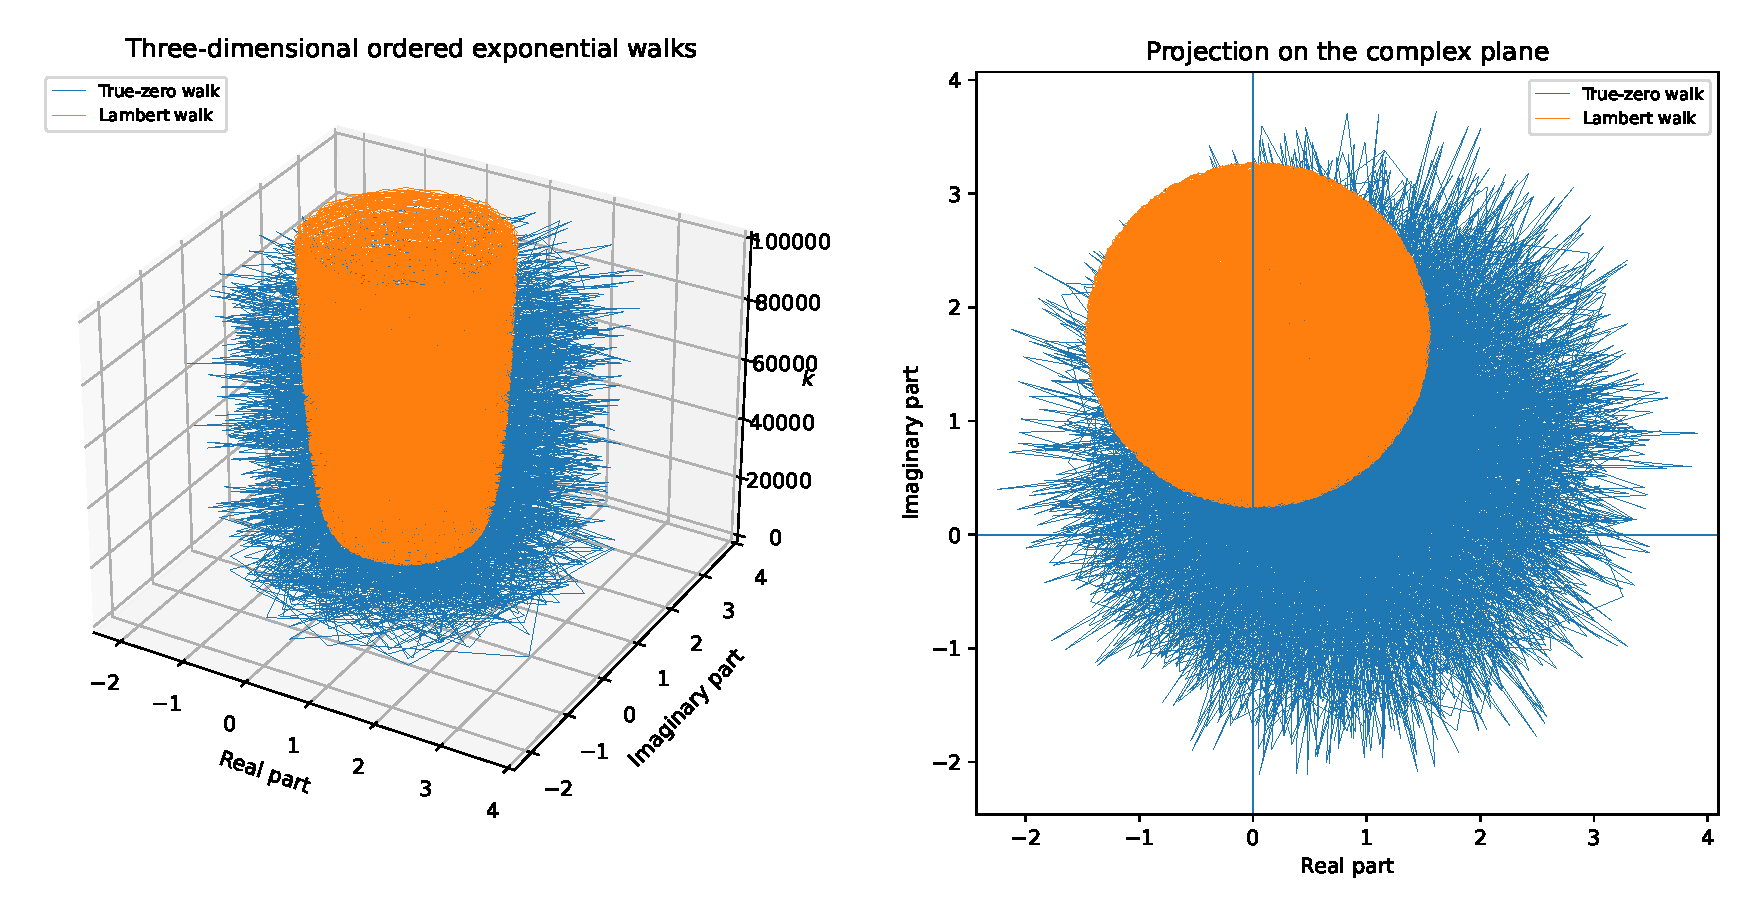
\includegraphics[width=0.98\textwidth]{figures/intro_zeta_vs_rvm_3d.pdf}
\par\smallskip
\small\textbf{Figure \thefigure.} Ordered exponential walks for the first $100{,}000$ ordinates. The left panel is the three-dimensional trajectory and the right panel is its projection onto the complex plane. The two curves are the true-zero walk $S_k^{\zeta}$ and the paired Lambert walk $S_k^{\mathrm{RVM}}$, shown on the same complex scale; the vertical coordinate in the three-dimensional panel is the ordinal index $k$.
\end{center}

\newpage
\begin{center}
\refstepcounter{figure}\label{fig:intro_paired_residual_3d}
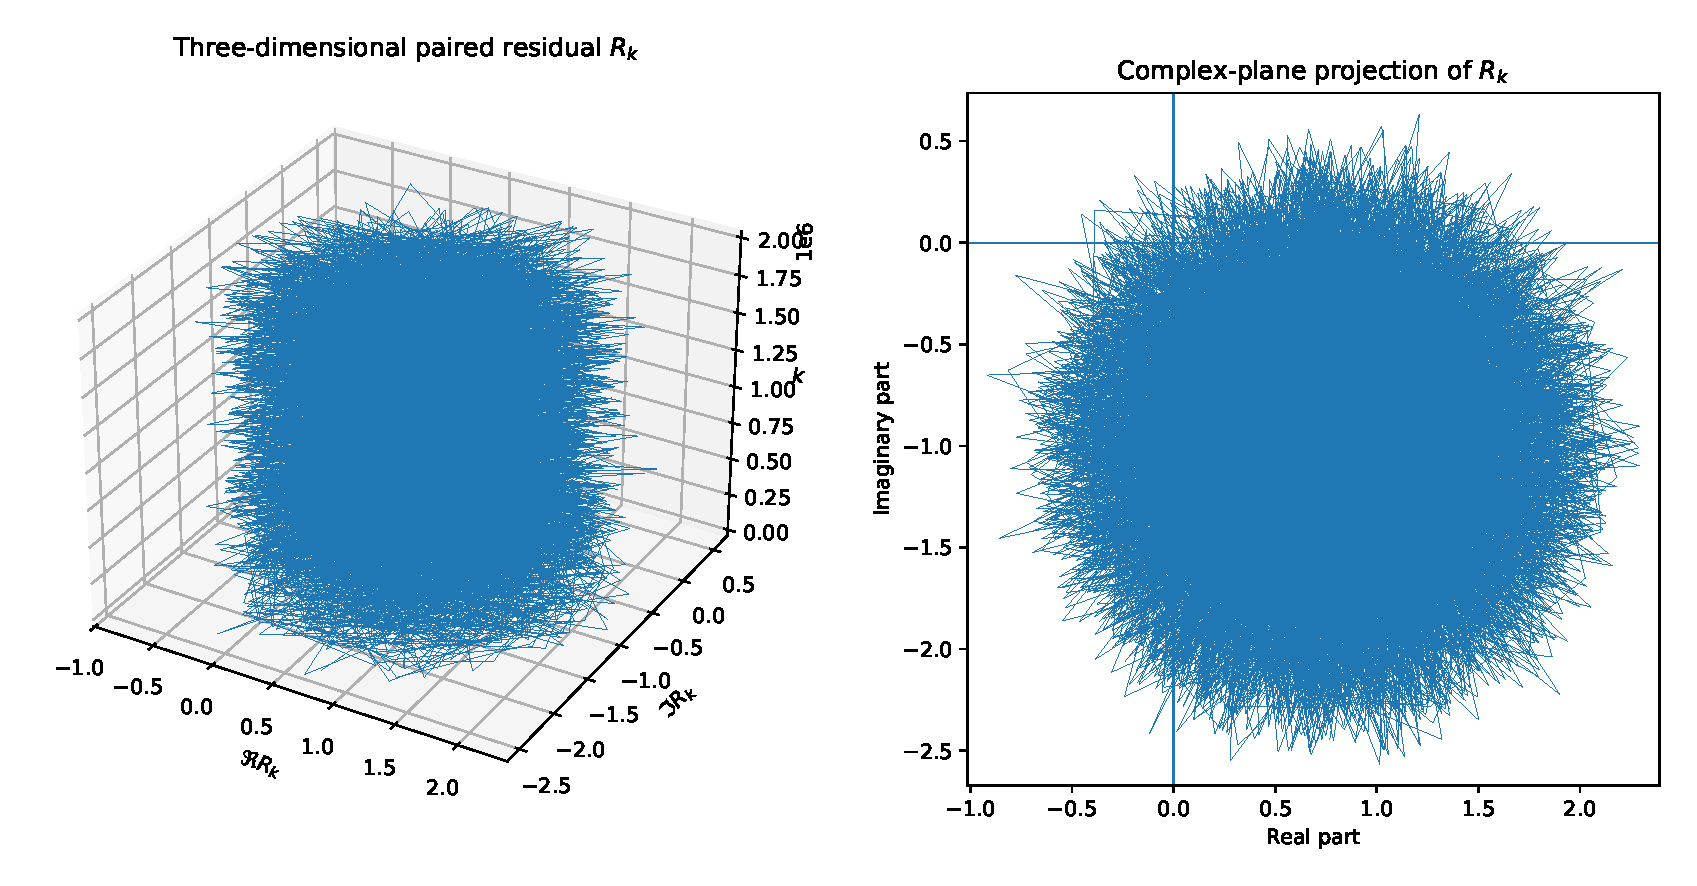
\includegraphics[width=0.70\textwidth]{figures/intro_paired_residual_3d.pdf}
\par\smallskip
\small\textbf{Figure \thefigure.} Paired residual obtained by subtracting after exponentiation: $R_k^{\mathrm{RVM}}=\sum_{j\le k}(e^{i\gamma_j}-e^{i\tau_j})$. The left panel is the three-dimensional trajectory and the right panel is its projection onto the complex plane. Over all $2{,}001{,}052$ pairs the observed path remains inside $|R_k^{\mathrm{RVM}}|\le3.0068262771$.
\end{center}

\newpage
\begin{center}
\refstepcounter{figure}\label{fig:intro_difference_before_exponential_3d}
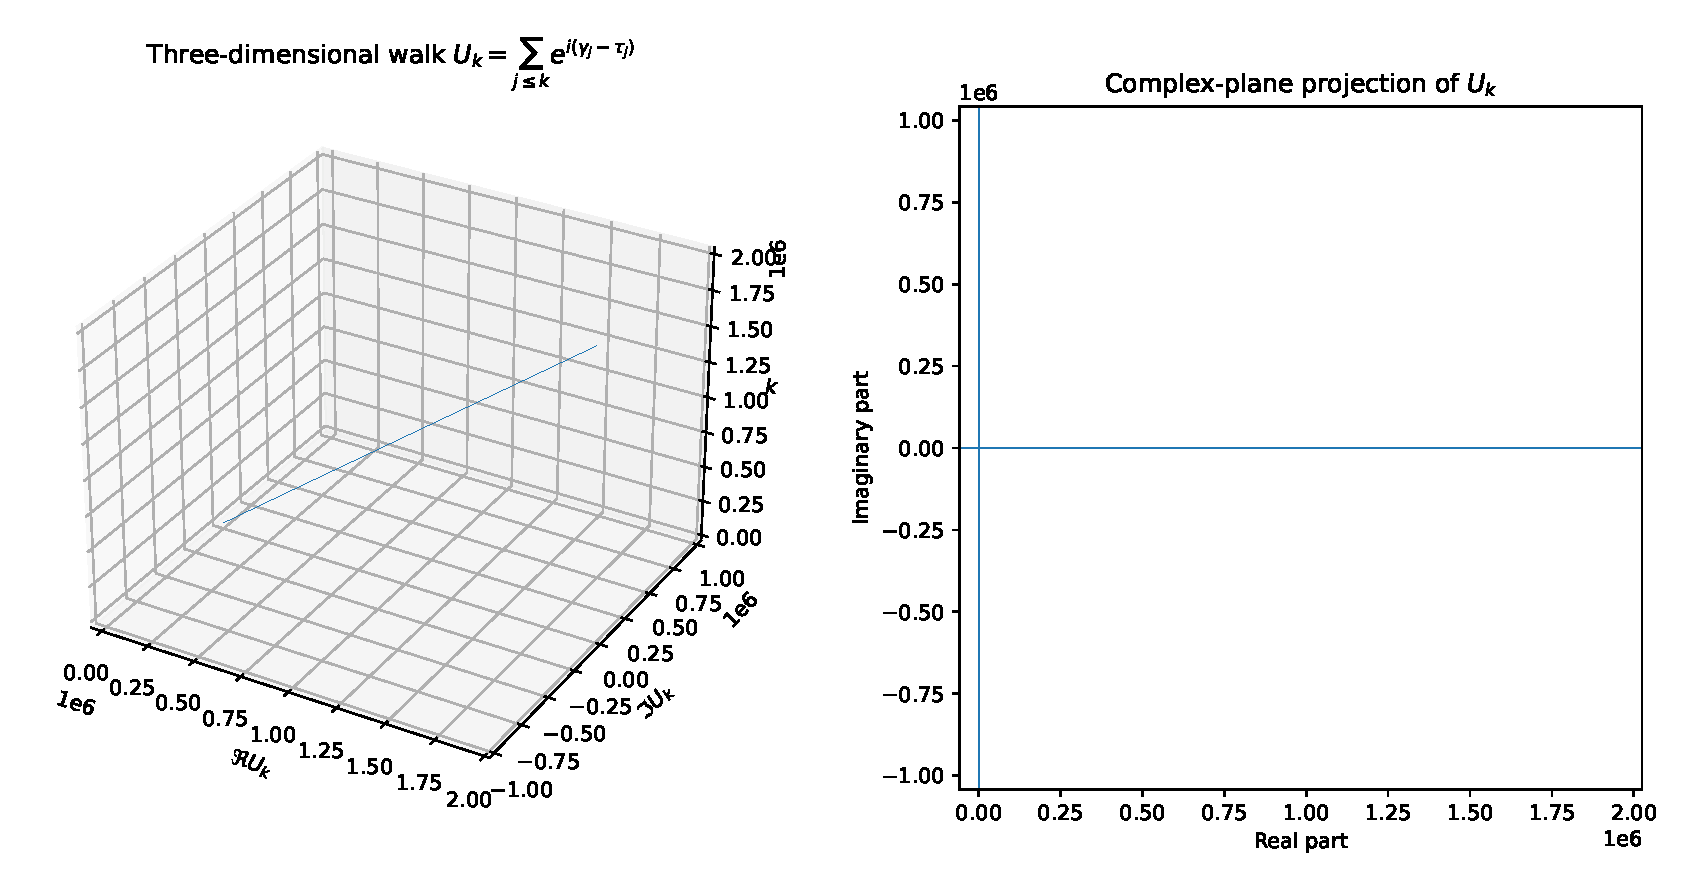
\includegraphics[width=0.70\textwidth]{figures/intro_difference_before_exponential_3d.pdf}
\par\smallskip
\small\textbf{Figure \thefigure.} Difference before exponentiation: $U_k^{\mathrm{RVM}}=\sum_{j\le k}e^{i(\gamma_j-\tau_j)}$. The left panel is the three-dimensional trajectory and the right panel is its projection onto the complex plane. This is not the same object as Figure~\ref{fig:intro_paired_residual_3d}; its centered version is $A_k^{\mathrm{RVM}}=U_k^{\mathrm{RVM}}-k$.
\end{center}

\newpage
\begin{center}
\refstepcounter{figure}\label{fig:intro_intrinsic_centered_residual_3d}
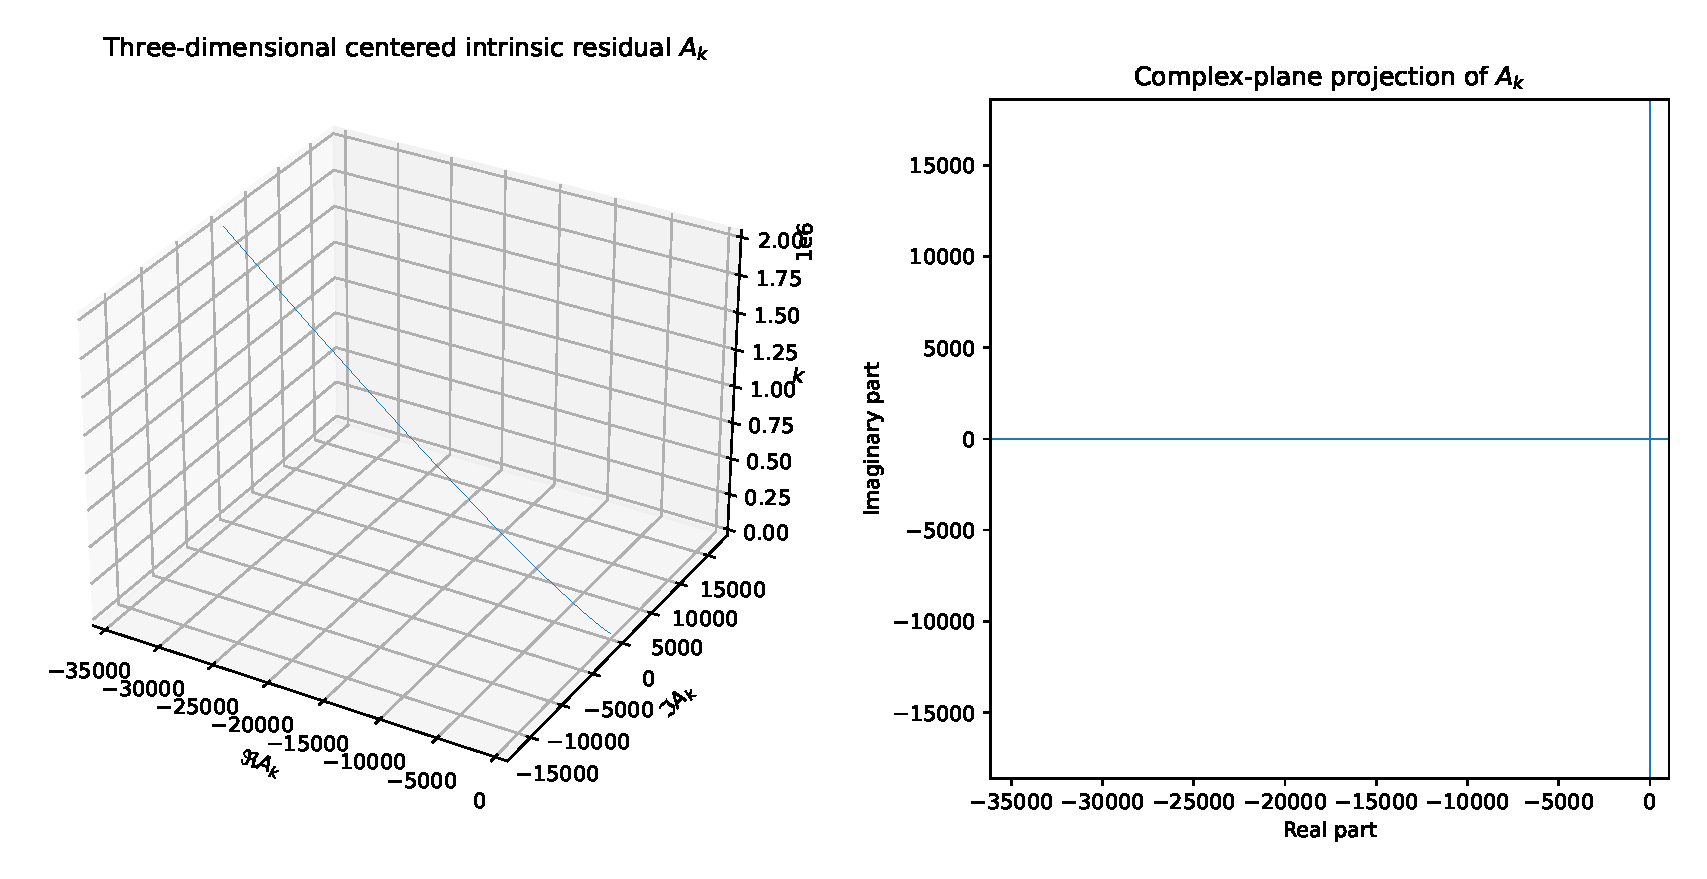
\includegraphics[width=0.88\textwidth]{figures/intrinsic_centered_residual_3d.pdf}
\par\smallskip
\small\textbf{Figure \thefigure.} Centered intrinsic residual: $A_k^{\mathrm{RVM}}=\sum_{j\le k}(e^{i(\gamma_j-\tau_j)}-1)$. The left panel is the three-dimensional trajectory and the right panel is its projection onto the complex plane.
\end{center}

The centroid is the first Cesàro mean of the endpoint sequence and, equivalently, a Riesz mean of order one relative to the ordinal frequency $\lambda_k=k-1$. The triangular factor is not a fixed cutoff that protects a finite prefix: for each fixed $k$, $1-(k-1)/N\to1$. Consequently, stabilization of $C_N^{\zeta}$ is a cancellation statement involving the whole expanding spectrum.

The frequency itself is special. The phase $e^{i\gamma}$ is the continuous Landau frequency $x=e$, because $x^{i\gamma}=e^{i\gamma}$ when $x=e$. Since $e$ is not an integral prime power, the leading fixed-$x$ prime-power resonance vanishes. Hlawka's equidistribution theorem gives $N^{-1}S_N^{\zeta}\to0$, while Ford--Zaharescu and Ford--Soundararajan--Zaharescu provide refined information on fixed multiples of zero ordinates and non-resonant secondary terms \cite{Hlawka,FordZaharescu2005,FordSoundZaha2009}. What those results do not directly evaluate is the order-one constant selected by the moving ordinal Cesàro kernel.

A distinction used throughout the paper is essential. Weighting the \emph{true} ordinates by the smooth counting clock, for example through
\begin{equation}\label{eq:intro_true_zero_landau}
\sum_{k=1}^{N}\left(1-\frac{M(\gamma_k)}{M(\gamma_N)}\right)e^{i\gamma_k},
\end{equation}
does not replace the ordinates by the Lambert levels $\tau_k$. Theorem~\ref{thm:truezerolandau} below shows that the statistic in \eqref{eq:intro_true_zero_landau} has the same asymptotic target as $C_N^{\zeta}$. Its numerical benchmark is therefore the zeta value $0.776907119554635+0.767844590760710\,i$, not the synthetic value $C_N^M$.

There are three layers to the answer.

First, the ordinal triangular centroid is superficially nonlinear in the zero-counting measure because the coefficient $N-k+1$ contains the rank $k$. The index is literal: if a positive ordinate $\gamma$ occurs with total upper-half-plane multiplicity $\nu(\gamma)$, then it occupies $\nu(\gamma)$ consecutive positions and every later index is shifted accordingly. On RH this includes ordinary multiplicity on the critical line; off RH it also includes the two upper-half-plane members $\beta+i\gamma$ and $1-\beta+i\gamma$ of each functional-equation pair, with their algebraic multiplicities. The lower conjugates at $-\gamma$ are not indexed. We therefore distinguish the midpoint argument term $S_*(\gamma)=\mathcal N_*(\gamma)-H(\gamma)$ from the individual ordinal defects
\[
r_k:=k-\frac12-H(\gamma_k).
\]
With
\[
H(x)=1+\frac{\vartheta(x)}{\pi},
\]
the exact decomposition is
\[
C_N^{\zeta}
=Q_N^{(H)}-\frac1N\sum_{k\leq N}r_ke^{i\gamma_k}.
\]
Over a complete ordinate block, the ordinal defects sum to $\nu(\gamma)$ times the midpoint argument value. This makes the Stieltjes analysis exact without assuming simplicity. We prove unconditionally that the normalized second term tends to zero. Thus the asymptotic centroid is reduced, without RH, to a linear statistic of the ordinates. This is the ``Level 1'' reduction in the terminology of the computational development.

Second, the synthetic smooth clock can be solved completely. For the main Riemann--von Mangoldt approximation
\[
M(x)=\frac{x}{2\pi}\log\frac{x}{2\pi e}+\frac78,
\]
the inverse ordinates are explicit through Lambert $W$. Their gaps are slowly decreasing and the associated phases admit a discrete Abel identity. Combining the first-derivative exponential-sum estimate with a second summation by parts proves convergence of the RVM centroid and yields a rapidly converging series for its limit. This is an unconditional theorem about the smooth model, independent of RH.

Third, evaluating the true zeta centroid by a holomorphic explicit formula introduces a different issue. An ordinary explicit formula naturally sees a zero $\rho=\beta+i\gamma$ through a holomorphic weight such as $e^{\rho-1/2}$, whereas the centroid uses the pure ordinate phase $e^{i\gamma}$. These coincide on the critical line. Off the line, functional-equation pairing produces the factor
\[
\cosh\!\left(\beta-\frac12\right).
\]
This is not an artefact of a particular contour; $e^{i\operatorname{Im}s}$ is not holomorphic. In particular, there cannot be a universal holomorphic kernel on the critical strip whose imaginary part is $\sin t$ independently of the real coordinate, because $\sin t$ is not harmonic as a function of $(\sigma,t)$.

This observation determines the precise role of RH. RH is not required to define $C_N$, nor to prove the unconditional Level 1 reduction. RH is required if one wants to replace the ordinate-only phase by the standard holomorphic complete-zero phase without retaining a horizontal defect. Under RH, a symmetric explicit-formula calculation at $x=e$ gives the closed real coordinate
\[
\frac{1}{2\sqrt e}\left(e-\frac1{e^2-1}\right).
\]
The underlying regularized bilateral identity is classical; the new point is its interpretation as the real coordinate of this particular ordinal triangular centroid, subject to the exact summability compatibility stated below.

The imaginary coordinate is one-sided. Pairing $+\gamma$ and $-\gamma$ removes it identically, so it cannot be recovered from the symmetric explicit formula alone. A one-sided transform of $S(t)$ produces instead a boundary value of $\Log\zeta$ with the two frequency branches $1+\log n$ and $1-\log n$. This is closely related in spirit to generalized Littlewood formulae and to the logarithmic-integral criteria of Sekatskii--Beltraminelli--Merlini \cite{Sekatskii2008,Sekatskii2009,Sekatskii2010}, but the present observable is an ordinal Cesàro transform rather than a fixed analytic test function. The exact bridge between those summation procedures is therefore stated as a separate boundary-interchange hypothesis rather than hidden inside the proof.

Finally, the horizontal defect connects the problem to a well-developed line of work. Fujii related antiderivatives of $S(t)$ to the positive quantity
\[
A_2(x)=\sum_{\substack{\beta>1/2\\0<\gamma\leq x}}
\left(\beta-\frac12\right)^2,
\]
and Bondarenko--Ivić--Saksman--Seip showed that this same horizontal mass governs the analytic continuation of the spectral zeta function
\[
G(s)=\sum_{\gamma>0}\gamma^{-s}
\]
beyond its unconditional half-plane \cite{Fujii2002,BondarenkoIvicSaksmanSeip2019}. The centroid defect begins with exactly this quadratic mass, but with an oscillatory factor $e^{i\gamma}$. At the boundary frequency $u=1$, zero-density estimates control its absolute mass but not the corresponding oscillatory value.

The organization is as follows. Sections~\ref{sec:prelim}--\ref{sec:riesz} set the counting and summability conventions. Section~\ref{sec:level1} proves the unconditional linearization. Section~\ref{sec:clockequiv} compares the exact Riemann--Siegel clock with its Lambert approximation. Section~\ref{sec:rvm} gives the unconditional RVM centroid theorem. Sections~\ref{sec:explicit}--\ref{sec:imaginary} derive the symmetric and one-sided explicit-formula values under precisely stated hypotheses. Section~\ref{sec:defect} isolates the off-critical-line defect. Section~\ref{sec:rh_equivalence} promotes the same centroid to the holomorphic family $C_N^{\zeta}(u)$ and proves the imaginary-axis equivalence with RH. Section~\ref{sec:fujii} relates the horizontal defect to Fujii's moment and the spectral zeta function. The final numerical section records the finite values, figures, and reproducibility checks.

\section{Preliminaries and conventions}\label{sec:prelim}

\subsection{Zeros, ordinal enumeration, multiplicity blocks, and the counting function}
Throughout the paper the ordinal index is
\[
\boxed{k=1,2,3,\ldots,N,}
\]
where \(k\) is the current zero index and \(N\) is only the final value of that same index in a finite truncation. We never use \(N\) as a second running index. Let
\[
\rho_k=\beta_k+i\gamma_k,\qquad \gamma_k>0,
\]
enumerate \emph{all} nontrivial zeros in the upper half-plane, counted with their individual algebraic multiplicities and ordered by nondecreasing ordinate. Thus
\[
0<\gamma_1\leq\gamma_2\leq\cdots\leq\gamma_N,
\]
and \(\gamma_1\) is literally the ordinate of the first upper-half-plane zero. The indices themselves are always distinct: there are never two equal values of \(k\). What can be equal are their ordinates, for example \(\gamma_k=\gamma_{k+1}\). Every repeated ordinate occupies a separate ordinal slot and therefore shifts every subsequent index. The conjugate zeros with ordinate \(-\gamma_k\) are not included in this enumeration.

For any positive zero ordinate \(\gamma\), define its \emph{upper-half-plane ordinate multiplicity}
\begin{equation}\label{eq:ordinate_multiplicity}
\nu(\gamma):=
\sum_{\substack{0<\beta<1\\ \zeta(\beta+i\gamma)=0}}
\operatorname{mult}(\beta+i\gamma).
\end{equation}
If
\[
a(\gamma):=\#\{k:\gamma_k<\gamma\},
\qquad
b(\gamma):=a(\gamma)+\nu(\gamma),
\]
then the whole ordinate block is
\begin{equation}\label{eq:ordinate_block_indices}
\gamma_{a(\gamma)+1}=\cdots=\gamma_{b(\gamma)}=\gamma.
\end{equation}
This convention treats multiplicity on and off the critical line without changing the indexing rule. On RH, a zero \(1/2+i\gamma\) of multiplicity \(m\) contributes \(m\) copies of the same ordinate \(\gamma\). Off the critical line, a zero \(\beta+i\gamma\), \(\beta\ne1/2\), of multiplicity \(m\) is accompanied by \(1-\beta+i\gamma\) with the same multiplicity, so the generic functional-equation pair contributes \(2m\) copies of the \emph{same positive ordinate} \(\gamma\). Their lower-half-plane conjugates contribute no additional indices here. Consequently every later ordinal index is shifted by the full upper-half-plane multiplicity actually present at preceding ordinates. The paired smooth level \(\tau_k\) is always attached to this actual ordinal index \(k\).

This is exactly where a conversion from a classical height cutoff to the ordinal cutoff must be handled with care. If a common ordinate occupies the consecutive slots
\[
\gamma_k=\gamma_{k+1}=\cdots=\gamma_{k+m-1}=\gamma,
\]
and a finite ordinal truncation ends inside that block, then a height cutoff at \(\gamma\) includes the \emph{entire} block, whereas the ordinal truncation includes only the slots up to \(N\). Therefore a height sum at \(\gamma_N\) is not identified term by term with a sum through \(k=N\) unless \(N\) is the last slot of its multiplicity block. The difference is precisely the uncompleted part of that one block. On the critical line a multiplicity-\(m\) zero creates \(m\) equal ordinates. Off the critical line a generic functional-equation pair of multiplicity \(m\) on each side creates \(2m\) equal positive ordinates. In both cases those repetitions are part of the ordinal numbering itself, not a secondary correction to it.

Let
\begin{equation}\label{eq:counting_function_mathcalN}
\mathcal N(x):=\#\{k:\gamma_k\le x\},
\end{equation}
so every zero is counted individually with algebraic multiplicity. At a zero ordinate \(\gamma\), let
\begin{equation}\label{eq:midpoint_count_mathcalN}
\mathcal N_*(\gamma)
:=\frac12\bigl(\mathcal N(\gamma^-)+\mathcal N(\gamma^+)\bigr)
=a(\gamma)+\frac{\nu(\gamma)}2.
\end{equation}
Define the Riemann--Siegel theta function
\[
\vartheta(x)=\operatorname{Im}\Log\Gamma\!\left(\frac14+\frac{ix}{2}\right)-\frac x2\log\pi,
\]
with its standard continuous determination for \(x>0\), and put
\[
H(x)=1+\frac{\vartheta(x)}{\pi}.
\]
Away from zero ordinates the Riemann--von Mangoldt formula is
\begin{equation}\label{eq:RVM_counting_mathcalN}
\mathcal N(x)=H(x)+S(x).
\end{equation}
At an ordinate \(\gamma\), define the midpoint argument value
\begin{equation}\label{eq:midpoint}
S_*(\gamma):=\mathcal N_*(\gamma)-H(\gamma).
\end{equation}
For every index \(a(\gamma)+j\) in the block, \(1\le j\le\nu(\gamma)\), put
\begin{equation}\label{eq:ordinal_defect_block}
r_{a(\gamma)+j}:=a(\gamma)+j-\frac12-H(\gamma).
\end{equation}
Then the complete-block identity is exact:
\begin{equation}\label{eq:ordinal_defect_block_sum}
\boxed{
\sum_{j=1}^{\nu(\gamma)}r_{a(\gamma)+j}
=\nu(\gamma)S_*(\gamma).}
\end{equation}
Thus Stieltjes jumps and ordinal weights agree on every complete ordinate block, whether that block comes from a multiple critical-line zero, an off-line functional-equation pair, or any combination of zeros sharing the same ordinate.

\begin{lemma}[Height-to-index transport with multiplicity]\label{lem:height_index_transport}
Uniformly for indices \(k\to\infty\),
\begin{equation}\label{eq:k_M_gamma_transport}
k=M(\gamma_k)+O(\log(2+\gamma_k)),
\end{equation}
and therefore
\begin{equation}\label{eq:k_gamma_asymp_transport}
k\asymp \gamma_k\log(2+\gamma_k),
\qquad
\gamma_k\asymp \frac{k}{\log(2+k)}.
\end{equation}
The estimates remain valid when \(k\) lies inside a multiplicity block.
\end{lemma}
\begin{proof}
For the block containing \(\gamma_k\), the index \(k\) lies between \(a(\gamma_k)+1\) and \(a(\gamma_k)+\nu(\gamma_k)\), hence
\[
|k-\mathcal N_*(\gamma_k)|\le \frac{\nu(\gamma_k)+1}{2}.
\]
The jump of \(\mathcal N\) at \(\gamma_k\) equals \(\nu(\gamma_k)\). Since \(H\) is continuous and the classical bound \(S(x)=O(\log(2+x))\) holds on both sides of the jump,
\begin{equation}\label{eq:ordinate_multiplicity_bound}
\nu(\gamma_k)=O(\log(2+\gamma_k)),
\qquad
S_*(\gamma_k)=O(\log(2+\gamma_k)).
\end{equation}
Thus \(\mathcal N_*(\gamma_k)=H(\gamma_k)+O(\log(2+\gamma_k))\). Using \(H(\gamma_k)=M(\gamma_k)+O(1/\gamma_k)\) gives \eqref{eq:k_M_gamma_transport}. The standard asymptotic form of \(M\) then gives \eqref{eq:k_gamma_asymp_transport}. No simplicity or RH assumption is used.
\end{proof}

\begin{remark}[How external height estimates are used]\label{rem:height_to_index_protocol}
The primary ordinal variable is \(k=1,2,\ldots,N\), with \(N\) used only for the final value of \(k\). Classical theorems stated with a continuous height cutoff are auxiliary inputs and are never converted by the formal substitution ``height \(=N\)''. For a finite endpoint \(N\), the relevant height is \(\gamma_N\), but if \(N\) lies inside a repeated-ordinate block then the classical cutoff at \(\gamma_N\) includes the full block while the ordinal sum does not. We therefore (1) apply the external theorem to the complete block at \(\gamma_N\); (2) remove the unused slots of that single endpoint block, counting their actual multiplicities; and only then (3) convert the height scale \(\gamma_N\) to the ordinal scale \(N\) by Lemma~\ref{lem:height_index_transport}. This protocol is used explicitly below for Hlawka/Ford--Zaharescu, Selberg, the Landau--Gonek formula, and Fujii's horizontal moment, and it is valid both for multiplicity on the critical line and for repeated positive ordinates produced by off-line functional-equation pairs.
\end{remark}

\begin{proposition}[Ordinal forms of the height estimates used below]\label{prop:ordinal_external_estimates}
With the enumeration and multiplicity convention above, the external height estimates used in this paper imply the following ordinal statements.
\begin{enumerate}[label=(\roman*)]
\item Hlawka's equidistribution theorem gives
\[
\sum_{k\le N}e^{i\gamma_k}=o(N).
\]
\item At the non-resonant frequency \(e^{i\gamma}\), the second-order Ford--Zaharescu theorem strengthens this to
\begin{equation}\label{eq:ordinal_FZ_rate}
\sum_{k\le N}e^{i\gamma_k}
=o\!\left(\frac{N}{\log N}\right).
\end{equation}
\item Selberg's height estimate
\[
\int_0^x S(t)^2\,\dd t\ll x\log\log x
\]
becomes, after evaluating at the endpoint ordinate and normalizing by \(N\),
\[
\frac{\gamma_N\log\log(2+\gamma_N)}{N}
=O\!\left(\frac{\log\log N}{\log N}\right)=o(1).
\]
\item Any complete-block error \(O(\log^A(2+x))\), with fixed \(A\), remains \(o(N)\) after passing to the possibly partial block containing \(\gamma_N\). In particular this applies to the local block corrections and to the \(H-M\) clock replacement used below.
\end{enumerate}
All sums in (i)--(iv) count the actual upper-half-plane zeros individually. Thus a critical-line zero of multiplicity \(m\) contributes \(m\) identical phases, while an off-line pair \(\beta+i\gamma\), \(1-\beta+i\gamma\), each of multiplicity \(m\), contributes \(2m\) identical ordinate phases \(e^{i\gamma}\). These repetitions are part of \(N\); they are not an error term and are never discarded in the height-to-index conversion.
\end{proposition}
\begin{proof}
For (i), Hlawka gives ordinary equidistribution of the fractional parts of \(\gamma/(2\pi)\), with zeros counted with multiplicity. Applied at the complete height cutoff \(\gamma_N\), the zero-mean test function \(e^{2\pi iu}\) gives a complete-block sum \(o(\mathcal N(\gamma_N))\). If \(N\) lies inside the terminal repeated-ordinate block, deleting the unused copies changes the sum by at most \(\nu(\gamma_N)=O(\log(2+\gamma_N))=o(N)\); hence the ordinal statement follows.

For (ii) we use precisely Corollary~2 of Ford--Zaharescu \cite{FordZaharescu2005}. Their second-order formula, valid for every \(f\in C^2(\mathbb T)\), is
\[
\sum_{0<\gamma\le \gamma_N} f(\alpha\gamma)
=\mathcal N(\gamma_N)\int_{\mathbb T}f
+\gamma_N\int_{\mathbb T} f(u)g_\alpha(u)\,\dd u
+o(\gamma_N),
\]
where the sum is the complete height sum and zeros are counted with multiplicity. Take
\[
f(u)=e^{2\pi iu},\qquad \alpha=\frac1{2\pi}.
\]
Then \(\int_{\mathbb T}f=0\). Moreover \(g_\alpha\equiv0\), because Ford--Zaharescu's resonant case requires \(\alpha=(a/q)\log p/(2\pi)\), whereas \(1=(a/q)\log p\) would imply \(e=p^{a/q}\), impossible. Thus
\begin{equation}\label{eq:FZ_complete_endpoint}
\sum_{0<\gamma\le\gamma_N}e^{i\gamma}=o(\gamma_N).
\end{equation}
This sum contains the \emph{whole} ordinate block at \(\gamma_N\). The ordinal sum \(\sum_{k=1}^N e^{i\gamma_k}\) may contain only part of that block; the difference has at most \(\nu(\gamma_N)=O(\log(2+\gamma_N))\) unit-modulus terms. Hence it is still \(o(\gamma_N)\). Finally Lemma~\ref{lem:height_index_transport} gives \(\gamma_N\asymp N/\log N\), proving \eqref{eq:ordinal_FZ_rate}. This argument is unchanged whether the repeated endpoint comes from a critical-line zero of multiplicity \(m\) or from an off-line pair, which contributes the corresponding repeated positive-ordinate slots.

Parts (iii) and (iv) follow directly from Lemma~\ref{lem:height_index_transport} and \eqref{eq:ordinate_multiplicity_bound}, with the same terminal-block correction when the ordinal cutoff ends inside a repeated ordinate.
\end{proof}

\subsection{The main smooth clock and Lambert inversion}
We shall also use
\begin{equation}\label{eq:Mclock}
M(x)=\frac{x}{2\pi}\log\frac{x}{2\pi e}+\frac78.
\end{equation}
The classical asymptotic expansion of $\vartheta$ gives
\begin{equation}\label{eq:HminusM}
H(x)=M(x)+\frac{1}{48\pi x}+O(x^{-3}).
\end{equation}
More terms and rigorous remainder estimates follow from the Stirling expansion for $\log\Gamma$; see, for example, Brent and Paris \cite{Brent2018,Paris2020}.

If $M(\tau_k)=k-\tfrac12$, then solving explicitly gives
\begin{equation}\label{eq:Lambertinverse}
\boxed{
\tau_k=\frac{2\pi(k-11/8)}{W_0((k-11/8)/e)}.
}
\end{equation}
We call $\{\tau_k\}$ the Lambert RVM clock. The exact smooth clock $\{\widehat\tau_k\}$ is defined instead by
\[
H(\widehat\tau_k)=k-\frac12.
\]
The two clocks are asymptotically close, but they are conceptually distinct.

\section{The exponential walk and its triangular Riesz mean}\label{sec:riesz}

\begin{definition}[Zeta exponential walk and centroid]
For the running ordinal index \(k=1,2,\ldots,N\), define
\[
S_k^{\zeta}:=\sum_{j=1}^{k}e^{i\gamma_j}.
\]
At the final index \(N\),
\[
S_N^{\zeta}=\sum_{k=1}^{N}e^{i\gamma_k},\qquad
C_N^{\zeta}:=\frac1N\sum_{k=1}^{N}S_k^{\zeta}.
\]
The symbol \(j\) is only a dummy summation variable inside the running partial sum; the zero positions themselves are indexed by \(k=1,\ldots,N\).
\end{definition}

\begin{proposition}[Exact triangular identity]\label{prop:triangle}
For every $N$,
\begin{equation}\label{eq:triangle}
\boxed{
C_N^{\zeta}
=\frac1N\sum_{k=1}^N(N-k+1)e^{i\gamma_k}
=\sum_{k=1}^N\left(1-\frac{k-1}{N}\right)e^{i\gamma_k}.
}
\end{equation}
\end{proposition}
\begin{proof}
In \(N^{-1}\sum_{k=1}^{N}S_k^{\zeta}\), the phase \(e^{i\gamma_j}\) occurs for \(k=j,j+1,\ldots,N\), hence exactly \(N-j+1\) times. Relabelling the dummy index \(j\) as \(k\) gives \eqref{eq:triangle}.
\end{proof}

\subsection{What the triangular weight does and does not do}
Equation~\eqref{eq:triangle} is the Cesàro $(C,1)$ mean of the partial sums. It is also a Riesz mean of order one relative to the ordinal frequency $\lambda_k=k-1$. For each fixed $k$,
\[
w_{k,N}:=1-\frac{k-1}{N}\longrightarrow1.
\]
Thus no fixed zero is suppressed in the limiting process. At a fixed $N$, zeros near the moving endpoint are attenuated; as $N$ grows, that attenuated region moves outward. This observation prevents a common misinterpretation of numerical stabilization: convergence can be fast while contributions continue to arrive from the entire spectrum, because convergence is produced by oscillatory cancellation rather than by permanent truncation of a tail.

The distinction also matters when comparing Riesz and Abel regularizations. The centroid uses the ordinal scale $k$, whereas an Abel factor $e^{-\varepsilon\gamma_k}$ regularizes in the height variable. Since
\[
k\sim \frac{\gamma_k}{2\pi}\log\gamma_k,
\]
the two kernels are not identical at the order-one scale. Any passage between them requires a Tauberian or boundary-interchange argument; it is not automatic.

\section{Unconditional elimination of the counting self-correlation}\label{sec:level1}

Define the linear exact-clock statistic
\begin{equation}\label{eq:QH}
Q_N^{(H)}
:=\frac1N\sum_{k=1}^N
\left(N+\frac12-H(\gamma_k)\right)e^{i\gamma_k}.
\end{equation}
By the definition of $r_k$ and \eqref{eq:triangle},
\begin{equation}\label{eq:exactCQ}
\boxed{
C_N^{\zeta}=Q_N^{(H)}-\frac1N\sum_{k=1}^N r_ke^{i\gamma_k}.
}
\end{equation}
The following theorem is the unconditional Level 1 statement.

\begin{theorem}[Unconditional Level 1]\label{thm:level1}
For a height \(x>0\) that is not a zero ordinate, define the complete-block sum
\begin{equation}\label{eq:Ax_definition}
A(x):=
\sum_{\substack{\gamma\le x\\ \gamma\ \mathrm{distinct}}}
\nu(\gamma)S_*(\gamma)e^{i\gamma}.
\end{equation}
Then
\begin{equation}\label{eq:Ax_bound}
A(x)=o(x\log x)
\qquad (x\to\infty).
\end{equation}
Consequently, in the primary ordinal variable,
\begin{equation}\label{eq:level1rate}
\boxed{
\frac1N\sum_{k=1}^N r_ke^{i\gamma_k}=o(1),
}
\end{equation}
and therefore
\begin{equation}\label{eq:CQlimit}
\boxed{C_N^{\zeta}-Q_N^{(H)}\longrightarrow0}
\end{equation}
unconditionally.
\end{theorem}

\begin{proof}
The proof is performed first at complete ordinate blocks and only then transported to the ordinal endpoint \(N\), as prescribed in Remark~\ref{rem:height_to_index_protocol}. As Stieltjes measures,
\[
\dd\mathcal N=\dd H+\dd S.
\]
Because the jump of \(\mathcal N\) at a distinct zero ordinate \(\gamma\) is exactly \(\nu(\gamma)\), the left side of \eqref{eq:Ax_definition} is precisely
\begin{align}
A(x)
&=\int_0^x e^{it}S_*(t)\,\dd\mathcal N(t)\notag\\
&=\int_0^x e^{it}S_*(t)\,\dd S(t)
 +\int_0^x e^{it}H'(t)S(t)\,\dd t+O(1).
\label{eq:Adecomp}
\end{align}
The midpoint convention gives the exact jump identity
\[
S_*\,\dd S=\frac12\,\dd(S^2).
\]
This remains exact for a jump of any size \(\nu(\gamma)\): in particular it covers a multiple zero on the critical line and an off-line functional-equation pair producing two or more copies of the same positive ordinate. Hence
\begin{equation}\label{eq:Aibp}
A(x)=
\frac12e^{ix}S(x)^2
-\frac{i}{2}\int_0^x e^{it}S(t)^2\,\dd t
+\int_0^x e^{it}H'(t)S(t)\,\dd t
+O(1).
\end{equation}

Selberg's unconditional second-moment theorem gives
\begin{equation}\label{eq:Selberg2}
\int_0^x S(t)^2\,\dd t\ll x\log\log x,
\end{equation}
so
\[
\int_0^x e^{it}S(t)^2\,\dd t=O(x\log\log x).
\]
The standard unconditional pointwise estimate \(S(x)=O(\log x)\) also gives \(e^{ix}S(x)^2=O(\log^2x)\).

For the linear term put
\begin{equation}\label{eq:Bheight_Fheight}
B(x):=\sum_{\gamma_k\le x}e^{i\gamma_k},
\qquad
F(x):=\int_0^x e^{it}S(t)\,\dd t,
\end{equation}
where the sum over \(k\) counts every upper-half-plane zero with its algebraic multiplicity. Since \(\dd S=\dd\mathcal N-H'(t)\dd t\), Stieltjes integration by parts gives
\begin{equation}\label{eq:Fidentity}
iF(x)
=e^{ix}S(x)-B(x)+\int_0^x e^{it}H'(t)\,\dd t+O(1).
\end{equation}
Write \(e^{i\gamma}=e^{2\pi i\alpha\gamma}\) with \(\alpha=(2\pi)^{-1}\). The input used here is exactly Corollary~2 of Ford--Zaharescu \cite{FordZaharescu2005}, not ordinary equidistribution. For every \(C^2\)-test function their formula contains the main term \(\mathcal N(x)\int f\), the secondary term \(x\int f g_\alpha\), and an \(o(x)\) remainder. With \(f(u)=e^{2\pi iu}\), the mean is zero; and \(g_\alpha\equiv0\) because \(\alpha=(2\pi)^{-1}\) is non-resonant. Consequently
\begin{equation}\label{eq:Bx_o_x}
B(x)=o(x)
\end{equation}
unconditionally. The sum \(B(x)\) is the complete height sum and counts every zero with algebraic multiplicity. Ordinary Hlawka equidistribution alone would give only \(o(\mathcal N(x))=o(x\log x)\) and would not suffice for the later ordinal rate.

Moreover \(H'(t)=O(\log t)\) and \(H''(t)=O(1/t)\), so
\[
\int_0^x e^{it}H'(t)\,\dd t=O(\log x),
\]
and \eqref{eq:Fidentity} yields
\begin{equation}\label{eq:Fbound}
F(x)=o(x).
\end{equation}
A further integration by parts gives
\begin{align}
\int_0^x e^{it}H'(t)S(t)\,\dd t
&=H'(x)F(x)-\int_0^x H''(t)F(t)\,\dd t+O(1)\\
&=o(x\log x).
\end{align}
Indeed, the endpoint is \(o(x\log x)\), while \(F(t)=o(t)\) and \(H''(t)=O(1/t)\) imply \(\int_0^xH''(t)F(t)\,\dd t=o(x)\). Substitution in \eqref{eq:Aibp} proves \eqref{eq:Ax_bound} for complete blocks.

Now fix an arbitrary ordinal endpoint \(N\). Let the block containing \(\gamma_N\) be \(a(\gamma_N)+1,\ldots,b(\gamma_N)\). Completing the possibly partial endpoint block changes \(\sum_{k\le N}r_ke^{i\gamma_k}\) by at most
\begin{equation}\label{eq:partial_block_level1_error}
O\!\left(\nu(\gamma_N)\bigl(|S_*(\gamma_N)|+\nu(\gamma_N)\bigr)\right)
=O(\log^2(2+\gamma_N)),
\end{equation}
by \eqref{eq:ordinate_multiplicity_bound}. The completed sum is \(A(\gamma_N)\) by \eqref{eq:ordinal_defect_block_sum}. Therefore
\[
\sum_{k=1}^N r_ke^{i\gamma_k}
=o(\gamma_N\log\gamma_N)+O(\log^2(2+\gamma_N)).
\]
Lemma~\ref{lem:height_index_transport} gives \(N\asymp\gamma_N\log(2+\gamma_N)\), so division by \(N\) proves \eqref{eq:level1rate}. Equation~\eqref{eq:CQlimit} follows from the exact identity \eqref{eq:exactCQ}.
\end{proof}

\begin{remark}
The theorem proves equality of the limiting behavior of $C_N^{\zeta}$ and $Q_N^{(H)}$; it does not, by itself, assert that either sequence converges. Convergence and evaluation of the limiting linear statistic require an additional argument.
\end{remark}

\section{Exact Riemann--Siegel clock versus Lambert clock}\label{sec:clockequiv}

Define the main-clock ordinal defect
\begin{equation}\label{eq:rM_definition}
r_k^{(M)}:=k-\frac12-M(\gamma_k).
\end{equation}
By \eqref{eq:HminusM},
\[
r_k^{(M)}=r_k+O(\gamma_k^{-1}).
\]
The zero-counting estimate $\mathcal N(x)\ll x\log x$ gives
\[
\sum_{\gamma_k\le x}\frac1{\gamma_k}\ll\log^2x.
\]
Therefore, at the ordinal endpoint $N$,
\begin{equation}\label{eq:HMphase}
\sum_{k\le N}
\bigl(r_k^{(M)}-r_k\bigr)e^{i\gamma_k}
=O(\log^2(2+\gamma_N))=o(N),
\end{equation}
where the last step follows from Lemma~\ref{lem:height_index_transport}. Repeated ordinates, whether caused by critical-line multiplicity or by off-line symmetry, are already included in the sum over $k$.

\begin{corollary}[Clock equivalence for Level 1]\label{cor:clocklevel1}
Replacing $H(\gamma_k)$ by $M(\gamma_k)$ in the linearization of Theorem~\ref{thm:level1} changes the normalized remainder by $o(1)$. Thus the exact Riemann--Siegel clock and the Lambert main clock are asymptotically equivalent for the Level 1 statement.
\end{corollary}

For the dataset of $N=2{,}001{,}052$ ordinates, the exact-clock linear statistic is
\[
Q_N^{(H)}
=0.776905882507509+0.767853218705326\,i,
\]
and the difference between the exact-$H$ and Lambert-$M$ versions is
\[
|Q_N^{(H)}-Q_N^{(M)}|=2.812\times10^{-10}.
\]
These finite values are numerical evidence only; Corollary~\ref{cor:clocklevel1} is the analytic asymptotic statement.

\subsection{The true-zero $M$-weighted Landau statistic}\label{subsec:true_zero_landau}

The smooth clock can be used as a weight while leaving the ordinates themselves unchanged. This is a different operation from replacing $\gamma_k$ by the Lambert levels $\tau_k$.

\begin{definition}[True-zero Landau-weighted statistic]\label{def:true_zero_landau}
For each ordinal endpoint $N$, put
\begin{equation}\label{eq:true_zero_landau}
L_N^{(M)}
:=\sum_{k=1}^{N}
\left(1-\frac{M(\gamma_k)}{M(\gamma_N)}\right)e^{i\gamma_k}.
\end{equation}
Also define
\begin{equation}\label{eq:QM_definition}
Q_N^{(M)}
:=\frac1N\sum_{k=1}^{N}
\left(N+\frac12-M(\gamma_k)\right)e^{i\gamma_k}.
\end{equation}
\end{definition}

\begin{theorem}[True-zero weighted target]\label{thm:truezerolandau}
One has, unconditionally,
\begin{equation}\label{eq:true_zero_landau_equivalence}
L_N^{(M)}-C_N^{\zeta}\longrightarrow0.
\end{equation}
Consequently, $L_N^{(M)}$ converges if and only if $C_N^{\zeta}$ converges, and in that case the two limits are equal.
\end{theorem}

\begin{proof}
Corollary~\ref{cor:clocklevel1} gives
\begin{equation}\label{eq:C_QM_equivalence}
C_N^{\zeta}-Q_N^{(M)}=o(1).
\end{equation}
Write
\begin{equation}\label{eq:Mend_definition}
M_N^{\mathrm{end}}:=M(\gamma_N)=N-\frac12-r_N^{(M)}.
\end{equation}
The standard pointwise bound for the argument term and \eqref{eq:HminusM} give
\begin{equation}\label{eq:Mend_asymptotic}
M_N^{\mathrm{end}}=N+O(\log(2+\gamma_N)).
\end{equation}
Let
\begin{equation}\label{eq:BN_AM_definitions}
B_N:=\sum_{k\leq N}e^{i\gamma_k},
\qquad
A_N^{(M)}:=\sum_{k\leq N}M(\gamma_k)e^{i\gamma_k}.
\end{equation}
Direct subtraction of \eqref{eq:true_zero_landau} and \eqref{eq:QM_definition} gives the exact identity
\begin{equation}\label{eq:LminusQM_exact}
L_N^{(M)}-Q_N^{(M)}
=\left(\frac1N-\frac1{M_N^{\mathrm{end}}}\right)A_N^{(M)}
-\frac{B_N}{2N}.
\end{equation}
At the fixed non-resonant frequency $x=e$, \eqref{eq:Bx_o_x} gives
\begin{equation}\label{eq:BN_index_bound}
B_N=o\!\left(\frac{N}{\log N}\right),
\end{equation}
because if $\gamma=\gamma_N$, completing the endpoint block changes $B_N$ by at most $\nu(\gamma)=O(\log(2+\gamma))$, while \eqref{eq:Bx_o_x} gives $o(\gamma)$ for the completed block and Lemma~\ref{lem:height_index_transport} gives $N\asymp\gamma_N\log(2+\gamma_N)$. This argument is unchanged if the block is enlarged by critical-line multiplicity or by an off-line functional-equation pair. Abel summation applied to the ordinal sequence $e^{i\gamma_k}$ therefore yields
\begin{equation}\label{eq:k_phase_bound}
\sum_{k\leq N}k e^{i\gamma_k}
=o\!\left(\frac{N^2}{\log N}\right).
\end{equation}
Since
\begin{equation}\label{eq:M_gamma_k_rank}
M(\gamma_k)=k+O(\log(2+\gamma_k)),
\end{equation}
we obtain, estimating the error term absolutely,
\begin{equation}\label{eq:AM_bound}
A_N^{(M)}
=o\!\left(\frac{N^2}{\log N}\right)+O(N\log N).
\end{equation}
Equations \eqref{eq:Mend_asymptotic}, \eqref{eq:BN_index_bound}, and \eqref{eq:AM_bound} inserted into \eqref{eq:LminusQM_exact} give
\begin{equation}\label{eq:LminusQM_o1}
L_N^{(M)}-Q_N^{(M)}=o(1).
\end{equation}
Combining this with \eqref{eq:C_QM_equivalence} proves \eqref{eq:true_zero_landau_equivalence}.
\end{proof}

\begin{remark}[The numerical target]\label{rem:true_zero_target}
For the run with $N=2{,}001{,}052$,
\begin{equation}\label{eq:zeta_target_numeric}
C_N^{\zeta}
=0.776907119554635+0.767844590760710\,i.
\end{equation}
The corresponding exact-clock statistic was
\begin{equation}\label{eq:QH_target_numeric}
Q_N^{(H)}
=0.776905882507509+0.767853218705326\,i,
\end{equation}
so
\begin{equation}\label{eq:finite_level1_gap}
\left|C_N^{\zeta}-Q_N^{(H)}\right|
=8.7162\times10^{-6}.
\end{equation}
Thus a closed-form candidate obtained from a weighted Landau calculation on the true zeros must be compared with \eqref{eq:zeta_target_numeric}; the synthetic Lambert centroid belongs to a different problem.
\end{remark}

\section{The RVM exponential centroid: an unconditional limit}\label{sec:rvm}

We now study a different object: the exponential walk generated by the synthetic Lambert ordinates $\tau_k$ themselves.

\begin{definition}
Let $\tau_k$ be given by \eqref{eq:Lambertinverse}. For the running index $k=1,\ldots,N$, define
\[
S_k^{M}:=\sum_{j=1}^{k}e^{i\tau_j},
\qquad
C_N^{M}:=\frac1N\sum_{k=1}^{N}S_k^M.
\]
Put
\[
g_k=\tau_{k+1}-\tau_k,
\qquad
v_k=e^{i\tau_k},
\qquad
 d_k=\frac1{e^{ig_k}-1}.
\]
\end{definition}

The identity
\[
v_k=d_k(v_{k+1}-v_k)
\]
is exact. Summing it gives the discrete Abel decomposition
\begin{equation}\label{eq:AbelSN}
S_N^{M}
=d_Nv_{N+1}-d_1v_1-
\sum_{k=1}^{N-1}(d_{k+1}-d_k)v_{k+1}.
\end{equation}

\begin{lemma}[Smooth-clock asymptotics]\label{lem:clockasym}
As $k\to\infty$,
\[
\tau_k\sim\frac{2\pi k}{\log k},\qquad
g_k\sim\frac{2\pi}{\log k},
\]
and
\[
d_k=-\frac{i}{g_k}-\frac12+O(g_k)=O(\log k),
\qquad
d_{k+1}-d_k=O(k^{-1}),
\]
with a second difference $\Delta^2d_k=O(k^{-2})$.
\end{lemma}
\begin{proof}
The first two estimates follow from inversion of $M$ and the inverse-function identity
\[
\tau'(x)=\frac1{M'(\tau(x))},\qquad
M'(t)=\frac1{2\pi}\log\frac{t}{2\pi}.
\]
The expansion
\[
\frac1{e^{ix}-1}=-\frac{i}{x}-\frac12+O(x)
\]
then yields the estimate for $d_k$. Differentiating the continuous interpolation $d(x)$ once and twice, using $\tau'(x)\asymp1/\log x$ and $\tau''(x)=O((x\log x)^{-1})$, gives the difference estimates by the mean-value theorem.
\end{proof}

\begin{lemma}[Smooth-clock exponential-sum bound]\label{lem:KL}
There is a constant $C$ such that
\[
\left|\sum_{k\le N}e^{i\tau_k}\right|\le C\log N.
\]
More generally, interval sums beginning at a sufficiently large index satisfy the corresponding first-derivative bound.
\end{lemma}
\begin{proof}
The continuous inverse $\tau(x)$ has positive monotone derivative
\[
\tau'(x)=\frac{2\pi}{\log(\tau(x)/(2\pi))}\asymp\frac1{\log x}.
\]
For large $x$, $0<\tau'(x)<2\pi$ and its distance from $2\pi\mathbb Z$ is bounded below by a constant multiple of $1/\log N$ on $[1,N]$. The Kusmin--Landau first-derivative estimate for exponential sums therefore gives $O(\log N)$. The finite initial segment is absorbed into the constant.
\end{proof}

\begin{theorem}[Existence and Abel series for the Lambert RVM centroid]\label{thm:RVMlimit}
The centroid $C_N^M$ converges. Its limit is
\begin{equation}\label{eq:RVMlimit}
\boxed{
C_M=-d_1e^{i\tau_1}
-\sum_{k=1}^{\infty}(d_{k+1}-d_k)e^{i\tau_{k+1}}.
}
\end{equation}
The series converges conditionally, and its tail satisfies
\begin{equation}\label{eq:RVMtail}
\sum_{k\ge J}(d_{k+1}-d_k)e^{i\tau_{k+1}}
=O\!\left(\frac{\log J}{J}\right).
\end{equation}
Moreover
\[
C_N^M-C_M=O\!\left(\frac{(\log N)^2}{N}\right).
\]
\end{theorem}
\begin{proof}
Let $q_k=d_{k+1}-d_k$. Lemma~\ref{lem:clockasym} gives $q_k=O(k^{-1})$ and $\Delta q_k=O(k^{-2})$, while Lemma~\ref{lem:KL} gives partial phase sums of order $O(\log k)$. Abel summation therefore yields
\[
\sum_{k\ge J}q_kv_{k+1}
=O\!\left(\frac{\log J}{J}\right),
\]
which proves convergence and \eqref{eq:RVMtail}.

Average \eqref{eq:AbelSN} over the running endpoint $k=1,\ldots,N$. One obtains the exact identity
\begin{equation}\label{eq:RVMcentroidAbel}
C_N^M
=-d_1v_1
+\frac1N\sum_{k=1}^N d_kv_{k+1}
-\sum_{k=1}^{N-1}\left(1-\frac{k}{N}\right)q_kv_{k+1}.
\end{equation}
A further Abel summation, now with $d_k=O(\log k)$ and the phase-sum bound, gives
\[
\frac1N\sum_{k\le N}d_kv_{k+1}=O\!\left(\frac{(\log N)^2}{N}\right).
\]
The difference between the weighted finite series in \eqref{eq:RVMcentroidAbel} and the infinite series in \eqref{eq:RVMlimit} is the sum of the tail \eqref{eq:RVMtail} and
\[
\frac1N\sum_{k<N}k q_kv_{k+1},
\]
which is $O(\log N/N)$ by Abel summation after the smooth asymptotic expansion. Together with the preceding boundary-average estimate this gives the stated $O((\log N)^2/N)$ rate and proves the theorem.
\end{proof}

\begin{remark}
The same strategy applies to the exact smooth clock $H(\widehat\tau_k)=k-\tfrac12$: its inverse derivative is again monotone with the same asymptotic scale, so an analogous Abel representation and convergence theorem follow. The closed Lambert formula \eqref{eq:Lambertinverse}, however, makes the $M$-clock version particularly transparent and directly reproducible.
\end{remark}

\section{The zeta centroid and the explicit formula}\label{sec:explicit}

The unconditional theorem \ref{thm:level1} reduces $C_N^{\zeta}$ to the linear statistic $Q_N^{(H)}$. Evaluation by a holomorphic explicit formula is a separate step.

\subsection{What non-resonance at $x=e$ removes}\label{subsec:nonresonance}
Landau's formula and its uniform refinements distinguish an integral prime power from a non-resonant fixed value of $x$ \cite{Landau1912,Gonek1993,FordZaharescu2005}. At $x=e$ one has $\Lambda(e)=0$, so the term of size $x$ supported at an exact prime-power resonance is absent. This fact is essential for the cancellation estimate used in Section~\ref{sec:level1}, but it is a statement at the leading height scale $x$.

Under RH, the uniform Landau formula of Ford--Zaharescu gives, for fixed $x=e$ and nearest integral prime power $n_e=3$,
\begin{equation}\label{eq:uniform_landau_e}
\sum_{\gamma_k\leq x}e^{i\gamma_k}
=-\frac{\log3}{2\pi\sqrt e}\,
\frac{e^{ix(1-\log3)}-1}{i(1-\log3)}
+O(\log^2 x).
\end{equation}
Equation \eqref{eq:uniform_landau_e} is not an evaluation of the order-one triangular centroid: its error term is larger than the displayed bounded contribution. Its role here is logical. The condition $\Lambda(e)=0$ removes the exact resonant term of order $x$; it does not imply that every lower-order arithmetic contribution to a one-sided or Cesàro-regularized value vanishes.

For an arbitrary ordinal endpoint $N$, complete the ordinate block containing $\gamma_N$. Under RH all zeros in that block lie on the critical line, but any algebraic multiplicity is still repeated in the index. Equation~\eqref{eq:uniform_landau_e} applied at the complete block, followed by the $O(\nu(\gamma_N))=O(\log(2+\gamma_N))$ partial-block correction, gives the purely ordinal consequence
\begin{equation}\label{eq:uniform_landau_ordinal}
\sum_{k\le N}e^{i\gamma_k}=O(\bigl(\log(2+N)\bigr)^2)
\qquad\text{under RH}.
\end{equation}
No zero is lost in this conversion: a critical-line zero of multiplicity $m$ contributes $m$ identical terms. Off-line blocks are irrelevant to \eqref{eq:uniform_landau_ordinal} because that displayed estimate is invoked under RH; the unconditional argument of Section~\ref{sec:level1} instead uses Ford--Zaharescu and the full upper-half-plane multiplicity convention.

\subsection{The symmetric real coordinate}\label{subsec:symmetric_real}
Let
\[
\Psi(u)=\psi(e^u),
\]
where $\psi$ is Chebyshev's function. The classical explicit formula may be written, with the usual symmetric regularization,
\begin{equation}\label{eq:explicitPsi}
\Psi(u)=e^u-
\sum_{\rho}^{\mathrm{reg}}\frac{e^{\rho u}}{\rho}
-\log(2\pi)-\frac12\log(1-e^{-2u}).
\end{equation}
Differentiating distributionally gives
\begin{equation}\label{eq:explicitDerivative}
\Psi'(u)=e^u-
\sum_{\rho}^{\mathrm{reg}}e^{\rho u}
-\frac{e^{-2u}}{1-e^{-2u}}.
\end{equation}
At $u=1$, the point $e^u=e$ is not an integer and hence is not a prime power; there is no Chebyshev atom at this point. Therefore
\begin{equation}\label{eq:regsumrho}
\boxed{
\sum_{\rho}^{\mathrm{reg}}e^{\rho}
=e-\frac1{e^2-1}.
}
\end{equation}
This identity is a classical consequence of the explicit formula. The centroid interpretation needs an additional summability identification.

\begin{hypothesis}[Symmetric Riesz compatibility at $u=1$]\label{hyp:SR}
The symmetric regularization in \eqref{eq:regsumrho}, after pairing $\rho$ and $\bar\rho$, agrees with the limit of the ordinal triangular Cesàro real statistic obtained from $Q_N^{(H)}$.
\end{hypothesis}

\begin{theorem}[Closed real coordinate]\label{thm:realconstant}
Assume RH and Hypothesis~\ref{hyp:SR}. Then the zeta centroid converges in real part and
\begin{equation}\label{eq:realclosed}
\boxed{
\lim_{N\to\infty}\Re C_N^{\zeta}
=\frac{1}{2\sqrt e}\left(e-\frac1{e^2-1}\right)
=0.77689426079325358\ldots.
}
\end{equation}
\end{theorem}
\begin{proof}
Under RH, every positive zero is $\rho=\tfrac12+i\gamma$, and its conjugate is $\bar\rho=\tfrac12-i\gamma$. Thus
\[
e^{\rho}+e^{\bar\rho}=2\sqrt e\cos\gamma.
\]
Pairing the zeros in \eqref{eq:regsumrho}, dividing by $2\sqrt e$, and applying Hypothesis~\ref{hyp:SR} yields the limit of the real triangular statistic. The unconditional Level 1 theorem transfers the same limit to $C_N^{\zeta}$.
\end{proof}

\begin{remark}[What is classical and what is specific]
Equation~\eqref{eq:regsumrho} is not presented as a new explicit formula. The specific assertion is the identification of its value with the real coordinate selected by the ordinal triangular centroid. That identification is exactly the content isolated in Hypothesis~\ref{hyp:SR}; it should not be conflated with the classical bilateral regularization itself.
\end{remark}

\section{One-sided transform and the full complex value}\label{sec:imaginary}

The imaginary coordinate cannot be recovered by pairing $+\gamma$ and $-\gamma$, because
\[
e^{i\gamma}+e^{-i\gamma}=2\cos\gamma.
\]
It requires a one-sided projection onto positive ordinates.

Fix $x_0\in(0,\gamma_1)$. For $\sigma>1$, define
\[
s_\sigma(t)=\frac1\pi\Im\Log\zeta(\sigma+it).
\]
By the Euler product,
\begin{equation}\label{eq:ssigma}
s_\sigma(t)
=-\frac1\pi\sum_{n\ge2}
\frac{\Lambda(n)}{n^\sigma\log n}\sin(t\log n).
\end{equation}
The one-sided triangular transform gives
\begin{equation}\label{eq:PsigmaPrime}
\cP_{\infty,\sigma}(x_0)
=
\frac{i e^{ix_0}}{2\pi}
\sum_{n\ge2}
\frac{\Lambda(n)}{n^\sigma\log n}
\left[
\frac{n^{ix_0}}{1+\log n}
-
\frac{n^{-ix_0}}{1-\log n}
\right].
\end{equation}
For $\sigma>1$ this is an absolutely justified rearrangement. Separating the slowly decaying $n=2$ term in the second branch yields the equivalent horizontal-$\Log\zeta$ formula
\begin{align}
\cP_{\infty,\sigma}(x_0)
=\frac{i e^{ix_0}}{2\pi}\Bigg\{&
\int_0^\infty e^{-u}\Log\zeta(\sigma+u-ix_0)\,\dd u\notag\\
&+\int_0^\infty e^u\left[
\Log\zeta(\sigma+u+ix_0)-2^{-(\sigma+u+ix_0)}
\right]\dd u\notag\\
&-\frac{2^{-\sigma-ix_0}}{1-\log2}
\Bigg\}.
\label{eq:PsigmaLogzeta}
\end{align}
The two denominators $1\pm\log n$ are the analytic record of the one-sided frequency split. Although $e$ itself is not a prime power, the one-sided projection contains nonlocal prime contributions; therefore the full complex centroid is not purely archimedean merely because the symmetric atom at $x=e$ vanishes.

\begin{remark}[The proposed arithmetic-free route]\label{rem:arithmetic_free_route}
There is a valid conditional implication but not a theorem of cancellation. If one could prove independently that
\begin{equation}\label{eq:prime_boundary_vanishes_hypothetically}
\lim_{\sigma\downarrow1/2}\cP_{\infty,\sigma}(x_0)=0,
\end{equation}
then the full constant in Theorem~\ref{thm:fullconstant} would reduce to the smooth term $\cB(x_0)$, which is built from the gamma factor and its derivatives. However, $\Lambda(e)=0$ does not imply \eqref{eq:prime_boundary_vanishes_hypothetically}. In the present one-sided representation the prime contribution is the entire series \eqref{eq:PsigmaPrime}, not a single atom at $n=e$. Moreover, the reproducibility evaluation at $x_0=1$ gives a nonzero boundary contribution
\begin{equation}\label{eq:prime_boundary_numeric}
\cP(1)=0.395112242469534+0.621692567335957\,i.
\end{equation}
Thus a reduction of the full complex centroid to a small list of archimedean constants would require a new cancellation identity not supplied by fixed-frequency non-resonance. The symmetric real coordinate is different: there the bilateral explicit formula at $u=1$ has no Chebyshev atom and yields the closed value in Theorem~\ref{thm:realconstant}.
\end{remark}

The smooth contribution is
\begin{equation}\label{eq:Bsmooth}
\cB(x_0)
=e^{ix_0}\bigl(H(x_0)+iH'(x_0)\bigr)
+i\int_{x_0}^{\infty}e^{it}H''(t)\,\dd t.
\end{equation}

\begin{hypothesis}[One-sided boundary interchange]\label{hyp:BI}
Assume that the finite ordinal triangular transform of the argument term may be passed to the critical-line boundary in the order
\[
N\to\infty,
\qquad \sigma\downarrow\frac12,
\]
so that the limiting one-sided arithmetic term equals
\[
\lim_{\sigma\downarrow1/2}\cP_{\infty,\sigma}(x_0),
\]
with the branch of $\Log\zeta$ obtained by continuation from $\Re s>1$. Equivalently, the relevant finite $S(t)$ transform and the regularized horizontal-$\Log\zeta$ transform have the same boundary value.
\end{hypothesis}

This hypothesis is the precise unresolved summability/contour interchange. It is deliberately separated from RH: RH controls the horizontal position of zeros, while Hypothesis~\ref{hyp:BI} controls the equality of two summation procedures.

\begin{theorem}[Conditional full complex centroid]\label{thm:fullconstant}
Assume RH and Hypothesis~\ref{hyp:BI}. Then $C_N^{\zeta}$ converges and, for every admissible $x_0\in(0,\gamma_1)$,
\begin{equation}\label{eq:Cfullformula}
\boxed{
C_\infty^{\zeta}
=\cB(x_0)+\lim_{\sigma\downarrow1/2}\cP_{\infty,\sigma}(x_0).
}
\end{equation}
For $x_0=1$, numerical evaluation of the zero-free right-hand side gives
\begin{equation}\label{eq:CstarNumeric}
\boxed{
C_\infty^{\zeta}=
0.77689426079325\ldots
+0.76785566886455\ldots\,i.
}
\end{equation}
Its real part agrees with the closed form \eqref{eq:realclosed}.
\end{theorem}
\begin{proof}
The exact Stieltjes decomposition behind Theorem~\ref{thm:level1} reduces the centroid to a smooth term and a linear transform of $S(t)$, while the quadratic term contributes $o(1)$ by Selberg's second moment. The smooth term tends to \eqref{eq:Bsmooth}. For $\sigma>1$, inserting \eqref{eq:ssigma} into the linear transform and integrating each sine mode gives \eqref{eq:PsigmaPrime}, equivalently \eqref{eq:PsigmaLogzeta}. Hypothesis~\ref{hyp:BI} authorizes passage to the critical-line boundary, and RH identifies the holomorphic complete-zero phase with the pure ordinate phase. The unconditional Level 1 theorem then transfers the result to the original centroid. The numerical value follows from direct quadrature of \eqref{eq:Bsmooth} and \eqref{eq:PsigmaLogzeta}; the accompanying Python script reproduces it without a table of zeta zeros.
\end{proof}

For reference, the reproducibility calculation at $x_0=1$ gives approximately
\[
\cB(1)=0.38178201832363+0.14616310152859\,i,
\]
\[
\cP(1)=0.395112242469534+0.621692567335957\,i,
\]
whose sum is \eqref{eq:CstarNumeric}.

\subsection{The holomorphic obstruction}\label{subsec:holomorphic_obstruction}
The role of RH can be stated without reference to any particular explicit formula.

\begin{proposition}[No universal holomorphic ordinate-phase kernel]\label{prop:nohol}
There is no holomorphic function $K$ on an open set containing a two-dimensional portion of the critical strip such that
\[
\Im K(\sigma+it)=\sin t
\]
independently of $\sigma$ throughout that open set.
\end{proposition}
\begin{proof}
The imaginary part of a holomorphic function is harmonic. But
\[
\Delta\sin t
=\frac{\partial^2}{\partial\sigma^2}\sin t
+\frac{\partial^2}{\partial t^2}\sin t
=-\sin t,
\]
which is not identically zero on any open set.
\end{proof}

Under RH, however,
\[
K(s)=e^{s-1/2}
\]
satisfies $K(\tfrac12+i\gamma)=e^{i\gamma}$. Thus RH is precisely what allows the standard holomorphic complete-zero weight to specialize to the pure ordinate phase at every nontrivial zero.

\section{The off-critical-line defect}\label{sec:defect}

Suppose $\rho=\tfrac12+\delta+i\gamma$ is paired by the functional equation with $\tfrac12-\delta+i\gamma$. The pure ordinate statistic assigns the pair the weight
\[
2e^{i\gamma},
\]
whereas the holomorphic complete-zero statistic gives
\[
e^{\delta+i\gamma}+e^{-\delta+i\gamma}
=2\cosh\delta\,e^{i\gamma}.
\]
The completed-minus-ordinate pair excess at the real boundary frequency $u=1$ is therefore
\begin{equation}\label{eq:pairdefect}
2(\cosh\delta-1)e^{i\gamma}.
\end{equation}

For a fixed functional-equation pair, the two ordinal triangular weights both tend to one as $N\to\infty$, regardless of how equal ordinates are ordered at finite $N$. Hence its completed-minus-ordinate contribution tends to \eqref{eq:pairdefect}. We do not identify the finite-$N$ paired difference with a single common triangular weight, because the two members of a tied pair may occupy different ordinal positions.

Two features are fundamental. First, Riesz tapering does not erase a hypothetical off-line zero at a fixed large height. The reason a zero extremely close to the critical line is hard to detect is instead the quadratic sensitivity
\begin{equation}\label{eq:quadraticdefect}
2(\cosh\delta-1)=\delta^2+O(\delta^4).
\end{equation}
For example, $\delta=10^{-6}$ produces a limiting pair amplitude of approximately $10^{-12}$.

Second, the limiting pair coefficients $2(\cosh\delta-1)$ are nonnegative but the phases $e^{i\gamma}$ are not. Consequently, vanishing of a regularized real-boundary excess at the isolated frequency $u=1$ would not force every coefficient to vanish: a positive discrete measure may have zero Fourier transform at one real frequency.

The cancellation issue at the real boundary frequency $u=1$ is resolved in a different way in Section~\ref{sec:rh_equivalence}: moving the \emph{same centroid family} to the positive imaginary axis converts the horizontal defect into a positive Laplace sum.



\section{A centroid-family equivalence to the Riemann hypothesis}\label{sec:rh_equivalence}

This section starts from the centroid itself and changes only its frequency parameter. The same triangular weights are used on both sides of the comparison. No smoothing of the zero sequence, contour evaluation, or boundary-interchange hypothesis enters the equivalence.

\subsection{Holomorphic realization of the ordinal centroid}\label{subsec:holomorphic_centroid_family}
For $u\in\mathbb C$ define
\begin{equation}\label{eq:centroid_frequency_family}
C_N^{\zeta}(u)
:=\frac1N\sum_{k=1}^{N}S_k^{\zeta}(u)
=\sum_{k=1}^{N}w_{k,N}e^{iu\gamma_k},
\qquad
S_k^{\zeta}(u):=\sum_{j=1}^{k}e^{iu\gamma_j},
\qquad
w_{k,N}=1-\frac{k-1}{N}.
\end{equation}
Thus $C_N^{\zeta}(1)=C_N^{\zeta}$. The real point $u=1$ belongs to the boundary of the half-plane used below.

\begin{theorem}[Holomorphic centroid in the upper frequency half-plane]\label{thm:holomorphic_centroid}
For every $u$ with $\Im u>0$, the limit
\begin{equation}\label{eq:centroid_upper_limit}
C^{\zeta}(u):=\lim_{N\to\infty}C_N^{\zeta}(u)
\end{equation}
exists and equals the absolutely convergent series
\begin{equation}\label{eq:centroid_upper_series}
\boxed{C^{\zeta}(u)=\sum_{k=1}^{\infty}e^{iu\gamma_k}.}
\end{equation}
For every compact $K\subset\{u:\Im u>0\}$,
\begin{equation}\label{eq:centroid_upper_rate}
\sup_{u\in K}|C_N^{\zeta}(u)-C^{\zeta}(u)|=O_K(N^{-1}).
\end{equation}
Consequently $C^{\zeta}$ is holomorphic on $\Im u>0$.
\end{theorem}

\begin{proof}
Let $y_K=\inf_{u\in K}\Im u>0$. Then
\begin{equation}\label{eq:centroid_phase_decay}
|e^{iu\gamma_k}|\le e^{-y_K\gamma_k}.
\end{equation}
The Riemann--von Mangoldt estimate $\mathcal N(x)\ll x\log x$ implies
\begin{equation}\label{eq:centroid_exp_moments}
\sum_{k\ge1}e^{-y_K\gamma_k}<\infty,
\qquad
\sum_{k\ge1}k e^{-y_K\gamma_k}<\infty.
\end{equation}
Using \eqref{eq:centroid_frequency_family} and \eqref{eq:centroid_upper_series},
\begin{equation}\label{eq:centroid_upper_difference}
C_N^{\zeta}(u)-C^{\zeta}(u)
=-\frac1N\sum_{k\le N}(k-1)e^{iu\gamma_k}
-\sum_{k>N}e^{iu\gamma_k}.
\end{equation}
The first term is bounded by
\[
\frac1N\sum_{k\le N}(k-1)e^{-y_K\gamma_k}
\le \frac1N\sum_{k\ge1}k e^{-y_K\gamma_k},
\]
and, since \(k/N\ge1\) for \(k>N\), the second term satisfies
\[
\sum_{k>N}e^{-y_K\gamma_k}
\le \frac1N\sum_{k>N}k e^{-y_K\gamma_k}.
\]
Thus
\[
\sup_{u\in K}|C_N^{\zeta}(u)-C^{\zeta}(u)|
\le \frac{2}{N}\sum_{k\ge1}k e^{-y_K\gamma_k}=O_K(N^{-1}),
\]
which proves \eqref{eq:centroid_upper_rate}. Local uniform convergence gives holomorphy by Weierstrass' theorem. Repeated ordinates cause no change: they appear as distinct ordinal slots \(k\), and the convergent majorant counts every such slot.
\end{proof}

The theorem is an interior statement. It does not identify the observed Riesz behavior at $u=1$ with an Abel or nontangential boundary value of $C^{\zeta}(u)$.

\subsection{The completed-zero centroid}\label{subsec:completed_zero_centroid}
Write the positive zeros as $\rho_k=\beta_k+i\gamma_k$, with the same multiplicities and ordinate ordering as in \eqref{eq:centroid_frequency_family}. Let
\begin{equation}\label{eq:xi_definition_centroid}
\xi(s):=\frac12s(s-1)\pi^{-s/2}\Gamma\!\left(\frac{s}{2}\right)\zeta(s),
\end{equation}
whose zeros are precisely the nontrivial zeros of $\zeta$, counted with multiplicity \cite{Titchmarsh1986,Edwards1974,DLMF}. Define
\begin{equation}\label{eq:completed_centroid_finite}
C_N^{\xi}(u):=\sum_{k=1}^{N}w_{k,N}e^{u(\rho_k-1/2)}.
\end{equation}
For $\Im u>0$ its limit is
\begin{equation}\label{eq:completed_centroid}
\boxed{C^{\xi}(u):=\lim_{N\to\infty}C_N^{\xi}(u)
=\sum_{\substack{\rho\\ \Im\rho>0}}e^{u(\rho-1/2)}.}
\end{equation}
The finite value in \eqref{eq:completed_centroid_finite} can depend on the arbitrary ordering of zeros sharing exactly the same ordinate, but its limit does not. This is the only place where the horizontal locations inside one fixed ordinate block can make the finite ordering visible: the ordinate centroid $C_N^{\zeta}(u)$ itself is insensitive to that ordering because all members of the block have the same $\gamma$. If RH holds, a multiplicity-$m$ zero on the line contributes $m$ identical completed terms. If RH fails, an off-line pair $\beta+i\gamma$, $1-\beta+i\gamma$, each with multiplicity $m$, occupies $2m$ ordinal positions at the same $\gamma$; after the complete pair is included its contribution is paired exactly as below. The convergence is absolute and locally uniform. Indeed, on a compact $K$ in the upper half-plane,
\begin{equation}\label{eq:completed_centroid_decay}
|e^{u(\rho-1/2)}|
\le e^{\frac12\sup_{u\in K}|\Re u|}e^{-y_K\gamma},
\end{equation}
and the same argument as in Theorem~\ref{thm:holomorphic_centroid} gives an $O_K(N^{-1})$ triangular-to-series error. Hence $C^{\xi}$ is holomorphic for $\Im u>0$.

\begin{remark}[Interior notation and the real boundary]\label{rem:completed_centroid_boundary}
The notation $C^{\xi}(u)$ is used only for $\Im u>0$, where the series in \eqref{eq:completed_centroid} converges absolutely. In particular, no quantity $C^{\xi}(1)$ is defined by that series in this paper. The conditional real-boundary limit $C_\infty^{\zeta}$ obtained in Theorem~\ref{thm:fullconstant} is a different object, defined through the ordinal centroid together with the stated boundary-interchange hypothesis. The RH equivalence below is entirely interior and does not use that hypothesis.
\end{remark}

\subsection{Positive imaginary-axis defect and RH}\label{subsec:positive_centroid_defect}
Functional-equation symmetry pairs
\begin{equation}\label{eq:functional_pair_same_ordinate}
\frac12+\delta_\rho+i\gamma
\quad\longleftrightarrow\quad
\frac12-\delta_\rho+i\gamma,
\qquad
\delta_\rho=\beta-\frac12.
\end{equation}
At $u=iy$, $y>0$, one simple off-line pair contributes $2e^{-y\gamma}$ to $C^{\zeta}(iy)$ and $2\cos(y\delta_\rho)e^{-y\gamma}$ to $C^{\xi}(iy)$. A pair of algebraic multiplicity $m$ contributes $m$ times these quantities. Critical-line multiplicities contribute equally to the two series and hence give zero defect. Therefore
\begin{equation}\label{eq:positive_imaginary_defect}
\boxed{
\mathcal D(y)
:=C^{\zeta}(iy)-C^{\xi}(iy)
=2\sum_{\substack{\beta>1/2\\\gamma>0}}
\left(1-\cos\!\left(y\left(\beta-\frac12\right)\right)\right)e^{-y\gamma}
\ge0.}
\end{equation}
The series converges absolutely for every $y>0$; the sum over $\beta>1/2$ counts algebraic multiplicity. Thus every off-line upper-half-plane functional-equation pair is represented exactly once on the right, with its multiplicity, while the ordinate series on the left contains both positive-ordinate members and therefore the same total ordinal count.

\begin{theorem}[Centroid-family equivalence with RH]\label{thm:centroid_RH_equivalence}
For every fixed $y_0$ with $0<y_0\le4\pi$,
\begin{equation}\label{eq:centroid_RH_equivalence}
\boxed{
\RH
\quad\Longleftrightarrow\quad
\mathcal D(y_0)=0
\quad\Longleftrightarrow\quad
C^{\zeta}(iy_0)=C^{\xi}(iy_0).}
\end{equation}
In particular,
\begin{equation}\label{eq:centroid_RH_equivalence_y1}
\boxed{\RH\quad\Longleftrightarrow\quad C^{\zeta}(i)=C^{\xi}(i).}
\end{equation}
\end{theorem}

\begin{proof}
If RH holds, $\delta_\rho=0$ for every nontrivial zero, so every term in \eqref{eq:positive_imaginary_defect} vanishes.

Conversely, suppose $\mathcal D(y_0)=0$. Equation~\eqref{eq:positive_imaginary_defect} is a convergent sum of nonnegative terms, so each term is zero. Hence
\begin{equation}\label{eq:cosine_zero_condition}
y_0\left(\beta-\frac12\right)\in2\pi\mathbb Z
\end{equation}
for every zero with $\beta>1/2$. Every nontrivial zero lies in the open strip $0<\beta<1$ \cite{Titchmarsh1986,DLMF}; therefore $|\beta-1/2|<1/2$. Since $0<y_0\le4\pi$,
\begin{equation}\label{eq:cosine_zero_range}
\left|y_0\left(\beta-\frac12\right)\right|<2\pi.
\end{equation}
The only multiple of $2\pi$ in this open interval is $0$, so $\beta=1/2$ for every nontrivial zero. This is RH.
\end{proof}

\begin{corollary}[RVM-residual form of the RH criterion]\label{cor:RVM_residual_RH_equivalence}
For $y>0$ define
\begin{align}
\mathcal R_{\mathrm{RVM}}(y)
&:=\sum_{k\ge1}e^{-y\tau_k}
\left(e^{-y(\gamma_k-\tau_k)}-1\right)
= C^{\zeta}(iy)-\sum_{k\ge1}e^{-y\tau_k},
\label{eq:RVM_residual_laplace}\\
\mathcal A_{\mathrm{RVM}}(y)
&:=C^{\xi}(iy)-\sum_{k\ge1}e^{-y\tau_k}.
\label{eq:RVM_arithmetic_archimedean_side}
\end{align}
Both series are absolutely convergent. The index $k$ is the actual upper-half-plane zero index from Section~\ref{sec:prelim}: if a positive ordinate is repeated because of algebraic multiplicity or an off-line functional-equation pair, the same $\gamma$ is repeated in the left series and the subsequent Lambert levels are shifted accordingly. There is exactly one $\tau_k$ for each actual ordinal slot. If RH fails, these repeated positive ordinates insert additional ordinal slots relative to an RH-only enumeration and therefore shift every subsequent pairing with $\tau_k$. Accordingly $\gamma_k-\tau_k$ is always an exact \emph{ordinally paired} Lambert residual; off RH it should not be interpreted as the displacement obtained by keeping the hypothetical RH indexing fixed. For every $y>0$,
\begin{equation}\label{eq:RVM_residual_inequality}
\boxed{\mathcal R_{\mathrm{RVM}}(y)\ge
\mathcal A_{\mathrm{RVM}}(y).}
\end{equation}
Moreover, for every fixed $y_0$ with $0<y_0\le4\pi$,
\begin{equation}\label{eq:RVM_residual_RH_equivalence}
\boxed{
\RH
\quad\Longleftrightarrow\quad
\mathcal R_{\mathrm{RVM}}(y_0)
=
\mathcal A_{\mathrm{RVM}}(y_0).}
\end{equation}
Equivalently,
\begin{equation}\label{eq:RVM_residual_RH_equivalence_expanded}
\boxed{
\RH
\quad\Longleftrightarrow\quad
\sum_{k\ge1}e^{-y_0\tau_k}
\left(e^{-y_0(\gamma_k-\tau_k)}-1\right)
=
C^{\xi}(iy_0)-\sum_{k\ge1}e^{-y_0\tau_k}.}
\end{equation}
\end{corollary}

\begin{proof}
Immediate from Theorem~\ref{thm:centroid_RH_equivalence}, since by construction
\begin{equation}\label{eq:RVM_residual_difference_is_defect}
\mathcal R_{\mathrm{RVM}}(y)-\mathcal A_{\mathrm{RVM}}(y)
=C^{\zeta}(iy)-C^{\xi}(iy)=\mathcal D(y).
\end{equation}
Thus \(\mathcal R_{\mathrm{RVM}}(y)\ge\mathcal A_{\mathrm{RVM}}(y)\), and equality at any fixed \(0<y_0\le4\pi\) is equivalent to \(\mathcal D(y_0)=0\), which is equivalent to RH by Theorem~\ref{thm:centroid_RH_equivalence}.
\end{proof}

The Lambert clock cancels algebraically from the difference in \eqref{eq:RVM_residual_difference_is_defect}. Its role is therefore not to supply an independent proof of RH, but to provide an explicit smooth reference that rewrites the positive centroid defect as a statement about the observed vertical residuals $\gamma_k-\tau_k$. At the real frequency $u=1$ the paired residual is a complex cancellation problem; on the positive imaginary axis the damped version is ordered by the nonnegative horizontal defect, and equality is exactly the RH criterion above.

The logical point is precise: the criterion starts from the same triangular centroid and embeds it in the complex-frequency family \eqref{eq:centroid_frequency_family}. It does not assert that the observed boundary value at $u=1$ alone is an RH criterion. The latter boundary identification remains the separate Riesz/Abel problem isolated in Sections~\ref{sec:riesz} and \ref{sec:imaginary}.

\begin{figure}[htbp]
\centering
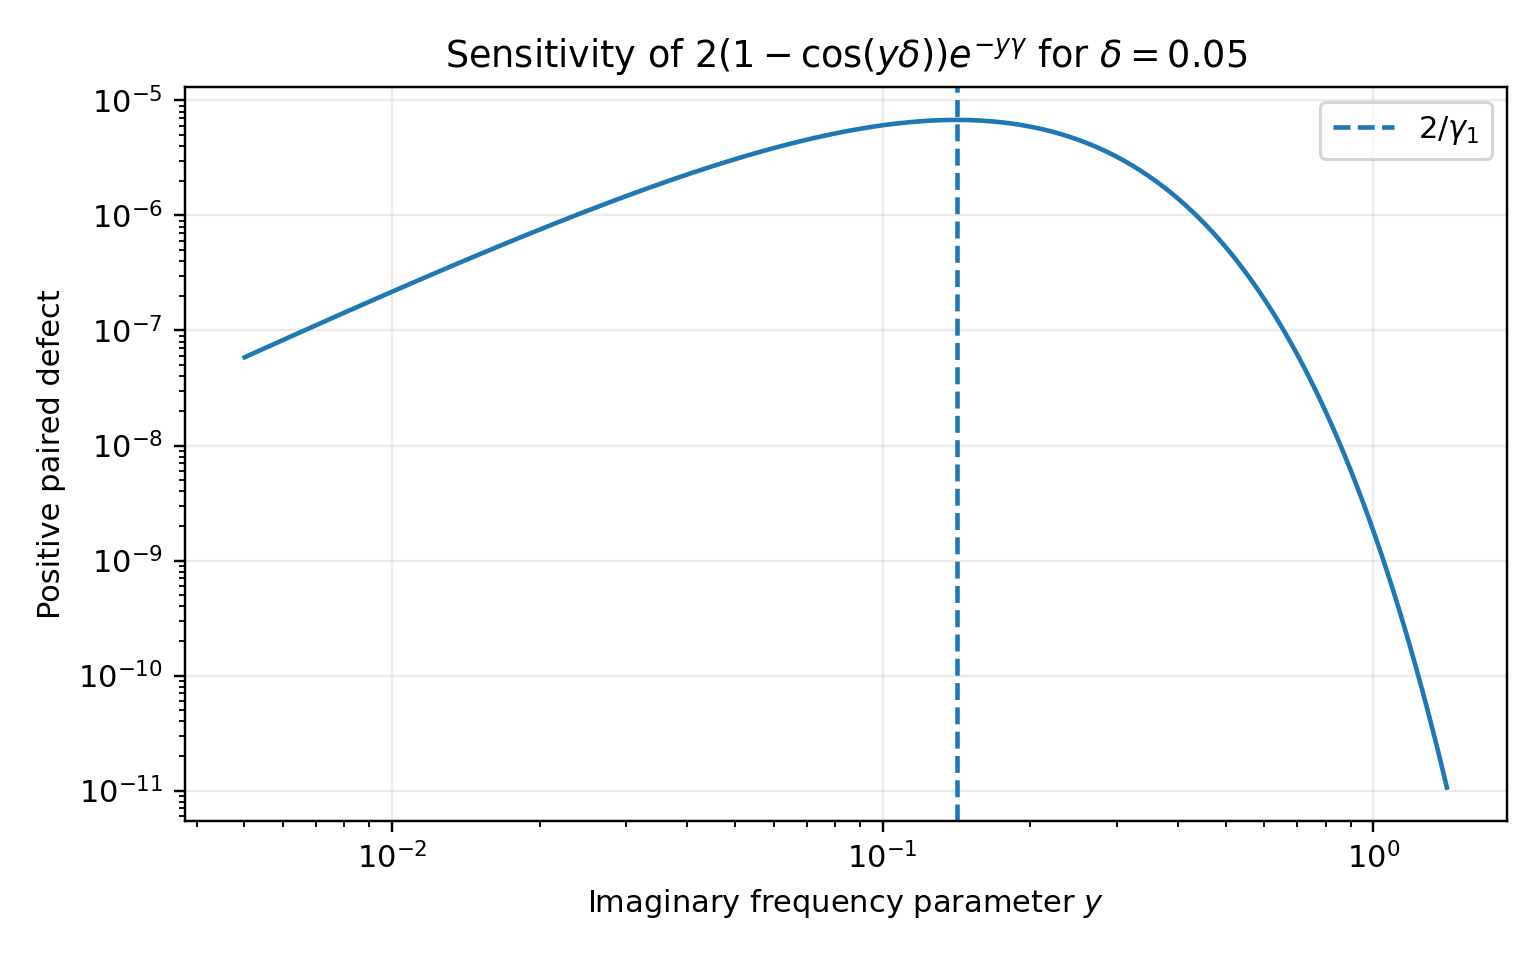
\includegraphics[width=0.82\textwidth]{rh_positive_defect_sensitivity.png}
\caption{Positive paired contribution to $\mathcal D(y)$ for the illustrative values $\delta_\rho=0.05$ and $\gamma=\gamma_1$: $2(1-\cos(y\delta_\rho))e^{-y\gamma}$. In the small-$y\delta_\rho$ regime the leading approximation is $y^2\delta_\rho^2e^{-y\gamma}$, whose maximum occurs near $y=2/\gamma$. The figure illustrates numerical sensitivity only; Theorem~\ref{thm:centroid_RH_equivalence} is exact.}
\label{fig:rh_positive_defect_sensitivity}
\end{figure}

\section{Fujii's horizontal moment and the spectral zeta function}\label{sec:fujii}

Define the horizontal second-moment counting function
\begin{equation}\label{eq:A2}
A_2(x)=
\sum_{\substack{\beta>1/2\\0<\gamma\le x}}
\left(\beta-\frac12\right)^2.
\end{equation}
Here zeros with $\beta>1/2$ are counted with algebraic multiplicity. The cutoff is deliberately a \emph{complete height cutoff}: for an off-line pair at ordinate $\gamma$, the member with $\beta>1/2$ enters together with all multiplicity copies at that ordinate. We do not identify $A_2(x)$ with a partially truncated ordinal sum inside an ordinate block, because such a truncation would depend on the arbitrary ordering of horizontally distinct zeros sharing the same $\gamma$. Whenever the endpoint is tied to the centroid index, the block containing $\gamma_N$ is completed first, exactly as in Remark~\ref{rem:height_to_index_protocol}.

Fujii proved an identity of the form
\begin{equation}\label{eq:Fujii}
\widetilde S_2(x)=A_2(x)+O(\log x),
\end{equation}
where $\widetilde S_2$ is an explicitly normalized second antiderivative quantity built from $S(t)$ \cite{Fujii2002}. Bondarenko--Ivić--Saksman--Seip use this relation in their study of
\[
G(s)=\sum_{\gamma>0}\gamma^{-s},
\]
showing unconditional meromorphic continuation to $\Re s>-1$ and relating further continuation to the horizontal distribution of zeros \cite{BondarenkoIvicSaksmanSeip2019}.

Our defect has the expansion
\[
2(\cosh\delta-1)
=\delta^2+\frac{\delta^4}{12}+\frac{\delta^6}{360}+\cdots.
\]
Since $0\le\delta<1/2$ for nontrivial zeros,
\[
1\le
\frac{2(\cosh\delta-1)}{\delta^2}
\le 8\left(\cosh\frac12-1\right)
=1.02100772\ldots.
\]
Thus Fujii's $A_2(x)$ is the leading positive mass underlying the exact horizontal defect. What the centroid needs, however, is not merely $A_2(x)$ but its oscillatory transform at frequency one:
\[
\int e^{it}\,\dd A_2(t).
\]
A zero-density or positive-mass estimate does not imply that this transform vanishes.

For $\Re s>1$ define
\[
H_2(s)=\sum_{\beta>1/2,\gamma>0}
\frac{(\beta-1/2)^2}{\gamma^s}.
\]
For $\Re z>0$, the Laplace transform of the horizontal mass has the Mellin representation
\begin{equation}\label{eq:MellinFujii}
F_2(z)
:=\sum_{\beta>1/2,\gamma>0}(\beta-\tfrac12)^2e^{-z\gamma}
=\frac1{2\pi i}\int_{(c)}\Gamma(s)z^{-s}H_2(s)\,\dd s,
\qquad c>1.
\end{equation}
The desired pure Fourier value is a boundary limit $z=\varepsilon-i$, $\varepsilon\downarrow0$. At that boundary the exponential decay of $\Gamma(c+it)$ is cancelled on one half of the contour by the factor $(-i)^{-s}$, which explains why the boundary is analytically more delicate than the damped Laplace regime. The Riesz kernel of the centroid does not remove this issue: it is a moving ordinal taper, not an exponential height damping.

This establishes the conceptual end point of the Fujii route at the real boundary frequency $u=1$. It identifies the exact positive horizontal mass responsible for the failure of the holomorphic ordinate projection, but a positive-mass estimate alone does not determine its oscillatory Fourier value there.

\section{Numerical values and reproducibility}\label{sec:numerics}

The analytic arguments above are independent of the numerical observations. This section records the finite values that motivated the analysis and the independent checks supplied with the manuscript.

\subsection{Finite true-zero and Lambert centroids}
For the dataset with
\[
N=2{,}001{,}052,
\qquad
\gamma_N\approx1{,}132{,}490.6587144111,
\]
the finite centroids are
\begin{align*}
C_N^{\zeta}
&=0.776907119554635+0.767844590760710\,i,\\
C_N^{\mathrm{Lamb}}
&=0.041570219277352+1.757541749592316\,i.
\end{align*}
The direct trajectory average and the triangular weighted formula agree to approximately $1.7\times10^{-13}$ for zeta and $4.9\times10^{-14}$ for the Lambert clock.

The conditional limiting value supplied by Theorem~\ref{thm:fullconstant} is
\[
C_\infty^{\zeta}=0.77689426079325\ldots+0.76785566886455\ldots i.
\]
At the available $N$, the real-coordinate discrepancy from the closed form is approximately
\[
1.29\times10^{-5}.
\]
No finite-$N$ observation is used as a premise in Theorem~\ref{thm:level1}, Theorem~\ref{thm:RVMlimit}, or the conditional explicit-formula derivations.

\subsection{Lambert-clock reproduction from the closed inverse}
The accompanying script \path{verify_rvm_centroid.py} reconstructs \eqref{eq:Lambertinverse} directly rather than reading the \texttt{zLamb.bin}. At $N=2{,}001{,}052$ it obtains
\[
C_N^M
=0.041570227040394+1.757541761467938\,i,
\]
with the Abel decomposition
\begin{align*}
-d_1e^{i\tau_1}
&=6.031991313792247+2.977851908778479\,i,\\
\frac1N\sum_{k\le N}d_ke^{i\tau_{k+1}}
&=-1.7006454064\times10^{-6}+1.3853445067\times10^{-7}i,\\
-\sum_{k<N}\left(1-\frac{k}{N}\right)\Delta d_ke^{i\tau_{k+1}}
&=-5.990419386106493-1.220310285845148\,i.
\end{align*}
The direct and Abel reconstructions differ by approximately $1.6\times10^{-13}$. The small difference from the Lambert centroid reflects the finite numerical generation of the smooth sequence rather than a change in definition.

\subsection{Zero-free evaluation of the conditional zeta constant}
The script \path{verify_zeta_conditional_constant.py} evaluates \eqref{eq:Bsmooth} and \eqref{eq:PsigmaLogzeta} at $x_0=1$ without reading a zeta-zero table. It gives
\begin{align*}
\cB(1)&=0.38178201832363+0.14616310152859\,i,\\
\cP(1)&=0.395112242469534+0.621692567335957\,i,\\
\cB(1)+\cP(1)&=0.77689426079317+0.76785566886455\,i.
\end{align*}
The independently evaluated real part differs from the closed expression \eqref{eq:realclosed} by about $9\times10^{-14}$ at the chosen numerical precision and tail truncation.


\subsection{Figures from the numerical tables}\label{subsec:numerical_figures}
The figures below are generated from the full-data tables and the reproducibility outputs listed in Appendix~\ref{sec:numerical_annex}. Their source CSV files and the plotting script are included in the accompanying package.

\begin{figure}[htbp]
\centering
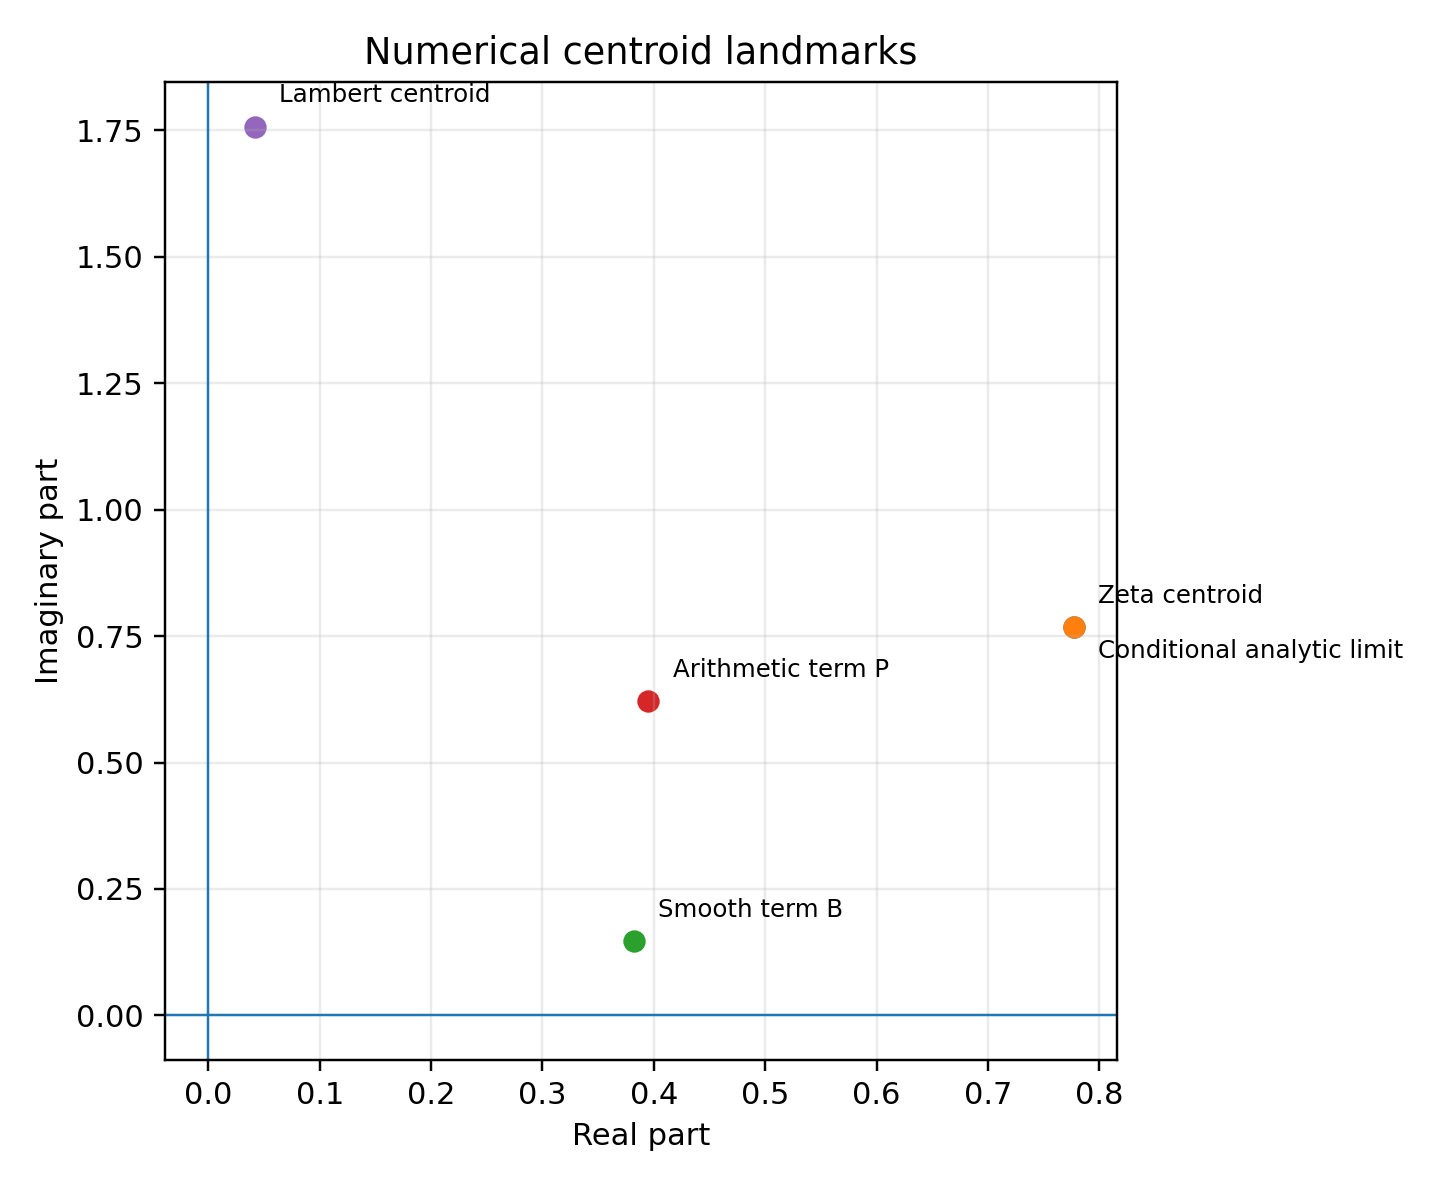
\includegraphics[width=0.86\textwidth]{centroid_complex_landmarks.png}
\caption{Finite and analytic complex landmarks: the zeta centroid, the Lambert centroid, the conditional analytic limit $C_\infty^{\zeta}$, and its smooth/arithmetic decomposition $\cB+\cP$.}
\label{fig:centroid_complex_landmarks}
\end{figure}

\begin{figure}[htbp]
\centering
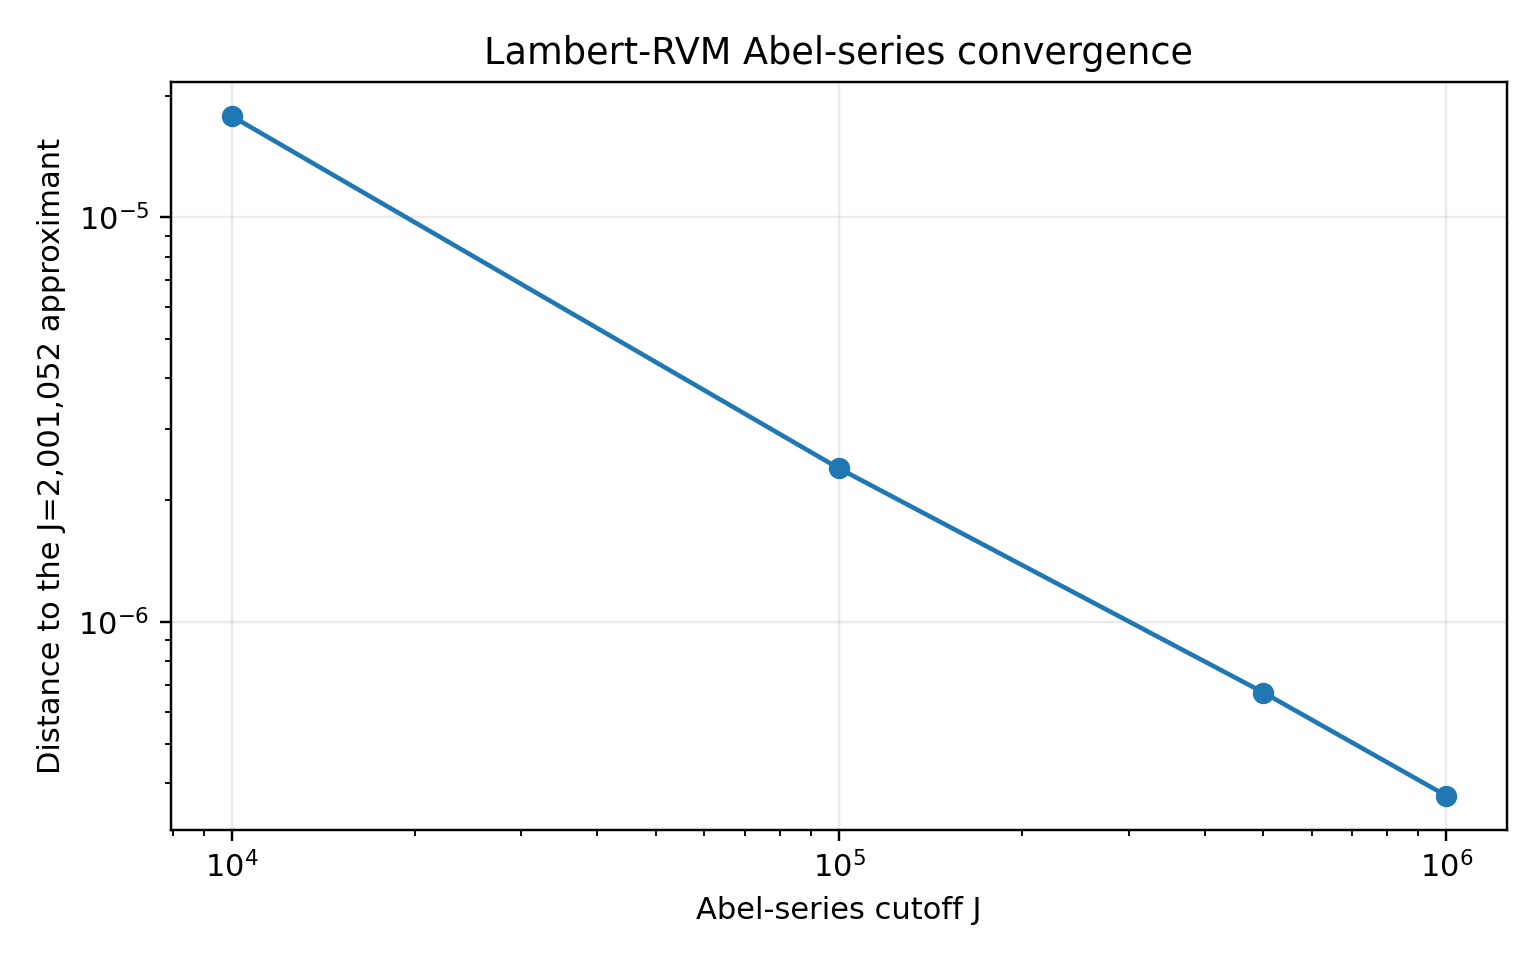
\includegraphics[width=0.86\textwidth]{rvm_abel_convergence.png}
\caption{Convergence of the Lambert-RVM unweighted Abel-series approximants recorded by \texttt{verify\_rvm\_centroid.py}. The ordinate is the distance from the largest cutoff $J=2{,}001{,}052$.}
\label{fig:rvm_abel_convergence}
\end{figure}

\begin{figure}[htbp]
\centering
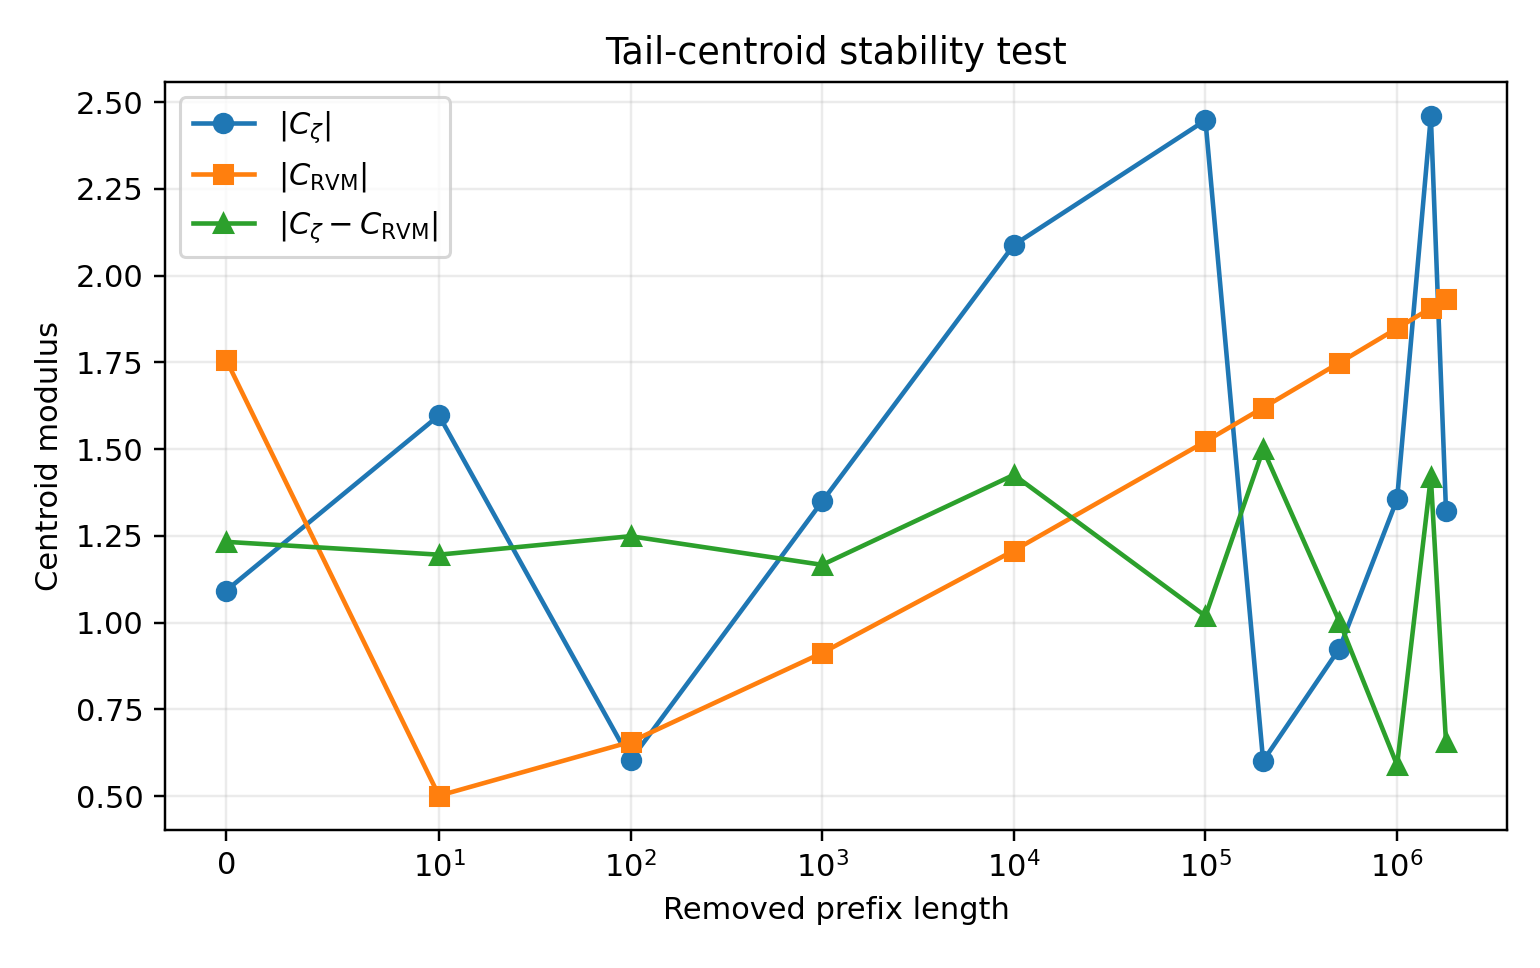
\includegraphics[width=0.86\textwidth]{tail_centroid_stability.png}
\caption{Tail-centroid test after deleting increasing prefixes of the true-zero and synthetic RVM sequences. The triangular taper does not permanently protect a finite prefix; the tail statistics remain of order one.}
\label{fig:tail_centroid_stability}
\end{figure}

\begin{figure}[htbp]
\centering
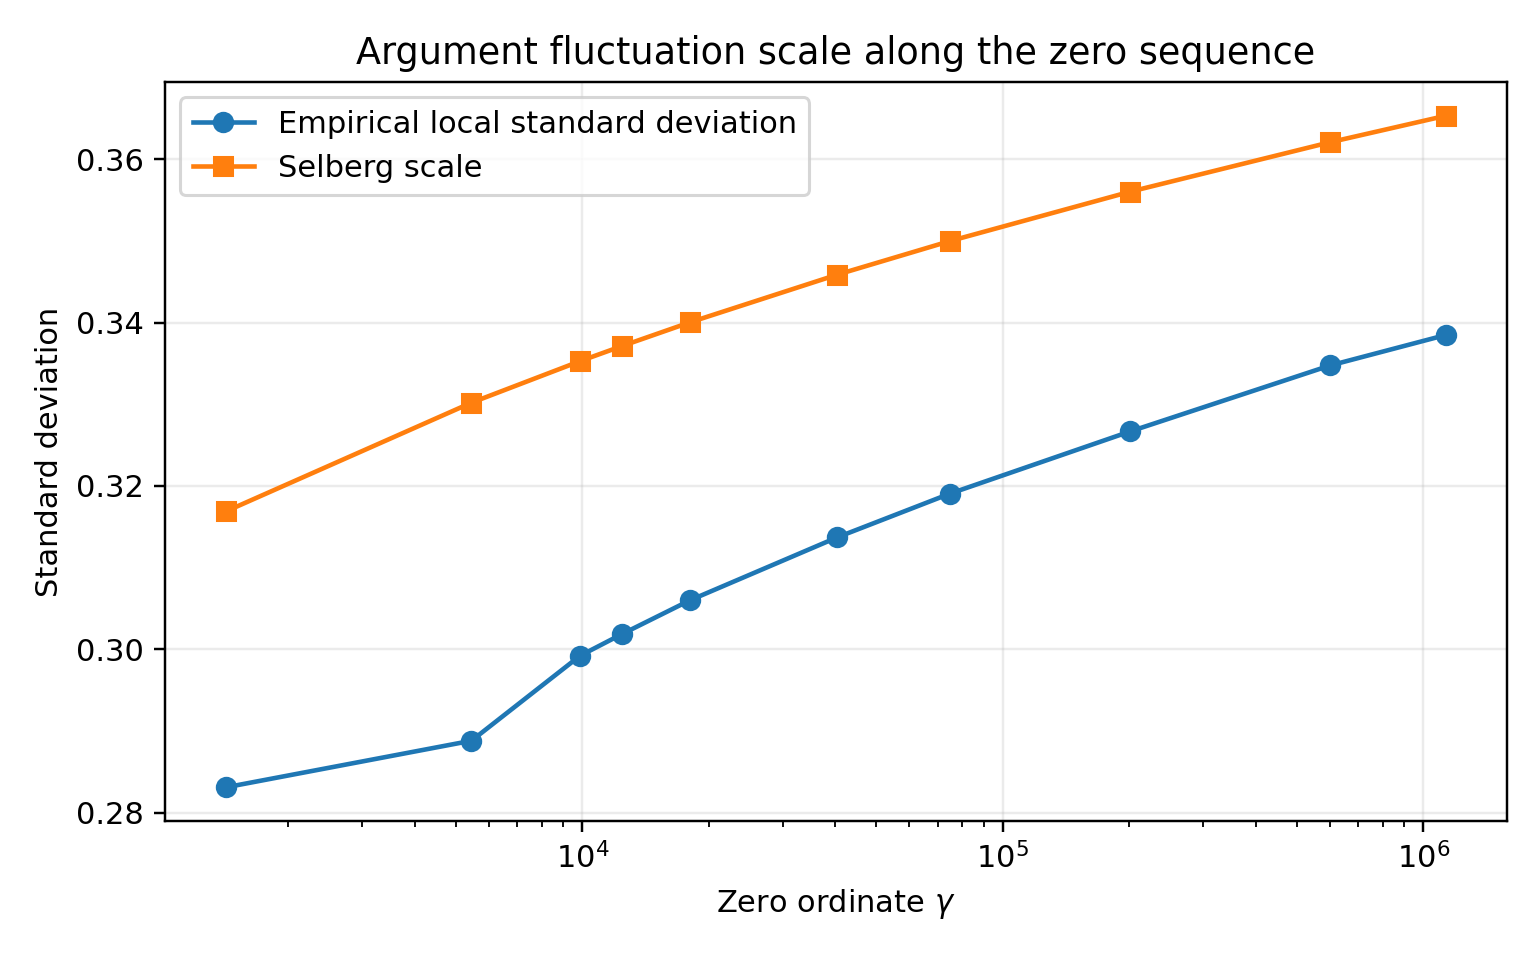
\includegraphics[width=0.86\textwidth]{argument_variance_profile.png}
\caption{Local standard deviation of the midpoint counting defect along the zero sequence compared with the Selberg scale used in the Level~1 analysis.}
\label{fig:argument_variance_profile}
\end{figure}

\section{Status of the main statements}\label{sec:status}

In the last column, ``None means that no conjectural or additional hypothesis is assumed. Published unconditional results used as inputs---for example Corollary~2 of Ford--Zaharescu in the Level~1 estimate---are cited in the relevant proofs and are not hypotheses of the statements.

\begin{center}
\small\begin{tabular}{@{}p{0.37\textwidth}p{0.18\textwidth}p{0.34\textwidth}@{}}
\toprule
Statement & Status & Required hypothesis \\
\midrule
Exact triangular centroid identity & Exact finite theorem & None \\
Unconditional Level 1, $C_N^{\zeta}-Q_N^{(H)}\to0$ & Proved & None \\
$H$ versus $M$ equivalence in Level 1 & Proved & None \\
True-zero weighted statistic $L_N^{(M)}-C_N^{\zeta}\to0$ & Proved & None \\
Lambert RVM centroid convergence and Abel series & Proved & None \\
Regularized bilateral identity at $u=1$ & Classical explicit formula & None for the regularized complete-zero identity \\
Closed real coordinate of the ordinal zeta centroid & Conditional theorem & RH + symmetric Riesz compatibility \\
Full complex limit $C_\infty^{\zeta}$ & Conditional theorem & RH + one-sided boundary interchange \\
Arithmetic-free full complex value from $\Lambda(e)=0$ alone & Not justified & Non-resonance removes only the leading prime-power atom \\
Off-line horizontal defect formula & Exact comparison & Functional-equation pairing \\
Holomorphic centroid $C^{\zeta}(u)$ for $\Im u>0$ & Proved & None \\
Centroid-family equality $C^{\zeta}(iy)=C^{\xi}(iy)$, $0<y\leq4\pi$ & Equivalent to RH & None \\
Boundary identification at $u=1$ & Separate summability problem & Riesz/Abel compatibility \\
\bottomrule
\end{tabular}
\end{center}

\section{Conclusions}\label{sec:conclusions}

The triangular exponential centroid admits a sharper analytic decomposition than is visible from its geometric definition. The rank-dependent coefficient can be separated into the exact Riemann--Siegel clock and the ordinal defect $r_k$; over complete multiplicity blocks the latter aggregates exactly to the midpoint argument term $S_*(\gamma)$. This self-correlation is negligible after normalization unconditionally. This converts the original centroid into a linear statistic without assuming RH.

The smooth RVM control is analytically complete: the Lambert inverse gives an exact model sequence, its exponential endpoint obeys a first-derivative cancellation estimate, and a discrete Abel transform yields a convergent series for the centroid limit. The triangular kernel is thereby seen correctly as a moving ordinal Riesz taper. It attenuates the finite upper edge but does not permanently suppress any fixed part of the spectrum.

The same smooth function $M$ can instead be used only as a weight on the true ordinates. Theorem~\ref{thm:truezerolandau} proves that this true-zero Landau-weighted statistic differs from $C_N^{\zeta}$ by $o(1)$. Its limiting target is therefore the zeta centroid, not the synthetic Lambert centroid. This removes a possible ambiguity between two constructions that share the same clock but not the same ordinates.

For the zeta centroid, the classical explicit formula at the non-prime-power frequency $x=e$ fixes a symmetric regularized complete-zero value. Under RH and the stated compatibility of that regularization with the ordinal triangular summation, this yields the closed real coordinate
\[
\frac{1}{2\sqrt e}\left(e-\frac1{e^2-1}\right).
\]
The full complex value requires a one-sided boundary transform. Its arithmetic part is naturally expressed through horizontal integrals of $\Log\zeta$ and contains the two branches $1\pm\log n$. The absence of an exact prime-power resonance at $x=e$ removes the leading Landau atom but does not annihilate this order-one one-sided arithmetic transform. The remaining mathematical issue is therefore not hidden: it is the boundary-interchange theorem that identifies this analytic one-sided regularization with the ordinal Cesàro limit.

Off the critical line, the real-boundary completed-minus-ordinate excess is controlled exactly by $2(\cosh(\beta-\tfrac12)-1)e^{i\gamma}$. Its leading horizontal sensitivity is quadratic, matching the positive mass isolated by Fujii and later used in the spectral-zeta analysis of Bondarenko--Ivić--Saksman--Seip. In the interior upper frequency half-plane, Theorem~\ref{thm:centroid_RH_equivalence} converts the same horizontal information into the nonnegative Laplace defect $\mathcal D(y)$ and gives the stated equivalence with RH. The boundary-value question at $u=1$ remains logically separate.

\begin{thebibliography}{99}

\bibitem{Riemann1859}
B.~Riemann,
\emph{Ueber die Anzahl der Primzahlen unter einer gegebenen Grösse},
Monatsberichte der Berliner Akademie (1859), 671--680.

\bibitem{Titchmarsh1986}
E.~C.~Titchmarsh, revised by D.~R.~Heath-Brown,
\emph{The Theory of the Riemann Zeta-Function}, 2nd ed.,
Oxford University Press, 1986.

\bibitem{Edwards1974}
H.~M.~Edwards,
\emph{Riemann's Zeta Function},
Academic Press, 1974; Dover reprint, 2001.

\bibitem{IwaniecKowalski2004}
H.~Iwaniec and E.~Kowalski,
\emph{Analytic Number Theory},
American Mathematical Society Colloquium Publications 53, 2004.

\bibitem{Ivic1985}
A.~Ivić,
\emph{The Riemann Zeta-Function: Theory and Applications},
Wiley, 1985; Dover reprint, 2003.

\bibitem{DLMF}
NIST Digital Library of Mathematical Functions,
\emph{Chapter 25: Zeta and Related Functions}, especially \S25.10,
\url{https://dlmf.nist.gov/25.10}.

\bibitem{Weyl1916}
H.~Weyl,
\emph{Über die Gleichverteilung von Zahlen mod. Eins},
Math. Ann. \textbf{77} (1916), 313--352.

\bibitem{Hlawka}
E.~Hlawka,
\emph{Über die Gleichverteilung gewisser Folgen, welche mit den Nullstellen der Zetafunktion zusammenhängen},
Sitzungsber. Österreich. Akad. Wiss. Math.-Naturwiss. Kl. Abt. II \textbf{184} (1975), 459--471.

\bibitem{Landau1912}
E.~Landau,
\emph{Über die Nullstellen der Zetafunktion},
Math. Ann. \textbf{71} (1912), 548--564,
DOI: 10.1007/BF01456808.

\bibitem{Gonek1993}
S.~M.~Gonek,
\emph{An explicit formula of Landau and its applications to the theory of the zeta-function},
in \emph{A Tribute to Emil Grosswald: Number Theory and Related Analysis},
Contemp. Math. \textbf{143}, American Mathematical Society, 1993, 395--413,
DOI: 10.1090/conm/143/1210528.

\bibitem{FordZaharescu2005}
K.~Ford and A.~Zaharescu,
\emph{On the distribution of imaginary parts of zeros of the Riemann zeta function},
J. Reine Angew. Math. \textbf{579} (2005), 145--158;
DOI: 10.1515/crll.2005.2005.579.145; arXiv:math/0405459.

\bibitem{FordSoundZaha2009}
K.~Ford, K.~Soundararajan and A.~Zaharescu,
\emph{On the distribution of imaginary parts of zeros of the Riemann zeta function, II},
Math. Ann. \textbf{343} (2009), 487--505;
DOI: 10.1007/s00208-008-0280-x; arXiv:0805.2745.

\bibitem{FordMengZaharescu}
K.~Ford, X.~Meng and A.~Zaharescu,
\emph{Simultaneous distribution of the fractional parts of Riemann zeta zeros},
arXiv:1511.06814.

\bibitem{Montgomery1973}
H.~L.~Montgomery,
\emph{The pair correlation of zeros of the zeta function},
Proc. Sympos. Pure Math. \textbf{24}, AMS, 1973, 181--193.

\bibitem{OdlyzkoTables}
A.~M.~Odlyzko,
\emph{Tables of zeros of the Riemann zeta function},
University of Minnesota, public numerical tables; the table of the first
$2{,}001{,}052$ zeros is documented as accurate to within $4\times10^{-9}$.
\url{https://www-users.cse.umn.edu/~odlyzko/zeta_tables/}.

\bibitem{Odlyzko1987}
A.~M.~Odlyzko,
\emph{On the distribution of spacings between zeros of the zeta function},
Math. Comp. \textbf{48} (1987), 273--308.

\bibitem{HughesRudnick2002}
C.~P.~Hughes and Z.~Rudnick,
\emph{Linear statistics for zeros of Riemann's zeta function},
C. R. Math. Acad. Sci. Paris \textbf{335} (2002), 667--670.

\bibitem{Selberg}
A.~Selberg,
classical unconditional second-moment results for $S(t)$ and $S_1(t)$;
see the historical account in Chirre--Quesada-Herrera \cite{ChirreQuesada2020}.

\bibitem{ChirreQuesada2020}
A.~Chirre and E.~Quesada-Herrera,
\emph{The second moment of $S_n(t)$ on the Riemann hypothesis},
arXiv:2006.08503.

\bibitem{Fujii2002}
A.~Fujii,
\emph{On the zeros of the Riemann zeta function},
Comment. Math. Univ. St. Pauli \textbf{51} (2002), no.~1, 1--17,
DOI: 10.14992/00008719.

\bibitem{Ivic2004}
A.~Ivić,
\emph{On certain sums over ordinates of zeta-zeros},
arXiv:math/0312303.

\bibitem{BondarenkoIvicSaksmanSeip2019}
A.~Bondarenko, A.~Ivić, E.~Saksman and K.~Seip,
\emph{On certain sums over ordinates of zeta-zeros II},
Hardy-Ramanujan J. \textbf{41} (2018/2019), 85--97;
arXiv:1808.01763.

\bibitem{Guinand}
A.~P.~Guinand,
classical explicit-formula work relating primes and zeros;
see Weil and modern treatments of the Guinand--Weil formula.

\bibitem{Weil1952}
A.~Weil,
\emph{Sur les ``formules explicites'' de la théorie des nombres premiers},
Comm. Sém. Math. Univ. Lund (1952), 252--265.

\bibitem{Barner}
K.~Barner,
\emph{On A. Weil's explicit formula},
J. Reine Angew. Math. \textbf{323} (1981), 139--152,
DOI: 10.1515/crll.1981.323.139.

\bibitem{Buthe2014}
J.~Büthe,
\emph{A method for proving the completeness of a list of zeros of certain $L$-functions},
Math. Comp. \textbf{84} (2015), 2413--2431; arXiv:1308.6704.

\bibitem{Sekatskii2008}
S.~K.~Sekatskii, S.~Beltraminelli and D.~Merlini,
\emph{A few equalities involving integrals of the logarithm of the Riemann zeta-function and equivalent to the Riemann hypothesis},
arXiv:0806.1596.

\bibitem{Sekatskii2009}
S.~K.~Sekatskii, S.~Beltraminelli and D.~Merlini,
\emph{A few equalities involving integrals of the logarithm of the Riemann zeta-function and equivalent to the Riemann hypothesis II},
arXiv:0904.1277.

\bibitem{Sekatskii2010}
S.~K.~Sekatskii, S.~Beltraminelli and D.~Merlini,
\emph{A few equalities involving integrals of the logarithm of the Riemann zeta-function and equivalent to the Riemann hypothesis III: exponential weight functions},
arXiv:1006.0323.

\bibitem{Brent2018}
R.~P.~Brent,
\emph{On asymptotic approximations to the log-Gamma and Riemann--Siegel theta functions},
J. Aust. Math. Soc. \textbf{107} (2019), 319--337;
arXiv:1609.03682.

\bibitem{Paris2020}
R.~B.~Paris,
\emph{Refined asymptotics of the Riemann--Siegel theta function},
arXiv:2004.00926.

\bibitem{Arias2014}
J.~Arias de Reyna,
\emph{On the distribution (mod 1) of the normalized zeros of the Riemann zeta-function},
J. Number Theory \textbf{153} (2015), 37--53; arXiv:1403.7126.

\bibitem{BrentPlattTrudgian2021}
R.~P.~Brent, D.~J.~Platt and T.~S.~Trudgian,
\emph{Accurate estimation of sums over zeros of the Riemann zeta-function},
Math. Comp. \textbf{90} (2021), 2923--2935, DOI: 10.1090/mcom/3652; arXiv:2009.13791.

\bibitem{Trudgian2014}
T.~S.~Trudgian,
\emph{An improved upper bound for the argument of the Riemann zeta-function on the critical line II},
J. Number Theory \textbf{134} (2014), 280--292; arXiv:1208.5846.

\end{thebibliography}


\appendix

\section{Numerical annex: full-data values}\label{sec:numerical_annex}
The centroid computation uses $N=2{,}001{,}052$ positive ordinates, with $\gamma_N\approx1.13249\times10^6$. The principal endpoint values are
\begin{align}
C_N^{\zeta}
&=0.776907119554635+0.767844590760710\,i,
\label{eq:annex_Czeta}\\
C_N^{\mathrm{Lamb}}
&=0.041570219277352+1.757541749592316\,i,
\label{eq:annex_CRVM}\\
Q_N^{(H)}
&=0.776905882507509+0.767853218705326\,i.
\label{eq:annex_QH}
\end{align}
The direct and triangular reconstructions agree to $1.73\times10^{-13}$ for the zeta centroid and $4.89\times10^{-14}$ for the RVM centroid. The midpoint counting defect has mean $4.22\times10^{-8}$, standard deviation $0.3321575$, and range approximately $[-1.33248,1.29937]$.

\subsection{Tail-centroid table}\label{subsec:annex_tail_centroid}
\begin{center}
\small
\begin{tabular}{rrrr}
\toprule
Removed prefix & $|C_\zeta|$ & $|C_{\rm RVM}|$ & $|C_\zeta-C_{\rm RVM}|$\\
\midrule
0 & 1.09230 & 1.75800 & 1.23300\\
10 & 1.59720 & 0.50157 & 1.19600\\
100 & 0.60399 & 0.65664 & 1.24920\\
1,000 & 1.34950 & 0.91298 & 1.16670\\
10,000 & 2.08820 & 1.20780 & 1.42590\\
100,000 & 2.44760 & 1.52210 & 1.01920\\
200,100 & 0.60171 & 1.61940 & 1.49940\\
500,260 & 0.92554 & 1.74910 & 1.00340\\
1,000,500 & 1.35580 & 1.84820 & 0.58972\\
1,500,800 & 2.45960 & 1.90640 & 1.41960\\
1,800,900 & 1.32320 & 1.93270 & 0.65554\\
\bottomrule
\end{tabular}
\end{center}

\subsection{Argument-fluctuation profile}\label{subsec:annex_argument_profile}
\begin{center}
\small
\begin{tabular}{rrr}
\toprule
$\gamma$ & empirical $\sigma$ & Selberg scale\\
\midrule
1,421.8 & 0.28310 & 0.31690\\
5,449.7 & 0.28880 & 0.33020\\
9,879.3 & 0.29921 & 0.33529\\
12,399.9 & 0.30184 & 0.33712\\
18,048.1 & 0.30601 & 0.34005\\
40,435.1 & 0.31372 & 0.34589\\
74,922.2 & 0.31907 & 0.35000\\
201,091.6 & 0.32669 & 0.35605\\
600,270.7 & 0.33476 & 0.36210\\
1,132,490.7 & 0.33850 & 0.36535\\
\bottomrule
\end{tabular}
\end{center}

\subsection{Lambert-RVM Abel approximants}\label{subsec:annex_rvm_abel}
\begin{center}
\small
\begin{tabular}{rcc}
\toprule
$J$ & real part & imaginary part\\
\midrule
10,000 & 0.041580072865611 & 1.757554793733856\\
100,000 & 0.041570891195329 & 1.757542207523970\\
500,000 & 0.041569346208409 & 1.757541422824472\\
1,000,000 & 0.041569178431353 & 1.757540990615438\\
2,001,052 & 0.041568808323635 & 1.757541025528465\\
\bottomrule
\end{tabular}
\end{center}

\subsection{Imaginary-axis sensitivity scale}\label{subsec:annex_rh_sensitivity}
For one hypothetical off-line pair with $\delta=0.05$ at the first ordinate $\gamma_1=14.134725142\ldots$, the positive defect is
\begin{equation}\label{eq:annex_pair_defect}
2(1-\cos(0.05y))e^{-y\gamma_1}.
\end{equation}
Its small-$y\delta$ approximation is $y^2\delta^2e^{-y\gamma}$ and is maximized at
\begin{equation}\label{eq:annex_yopt}
y_{\rm opt}\approx\frac{2}{\gamma},
\end{equation}
which gives $y_{\rm opt}\approx0.1414955$ at $\gamma_1$.
The direct pairwise values used to check the sign and scale are
\begin{center}
\small
\begin{tabular}{rcc}
\toprule
$y$ & $e^{-y\gamma_1}$ & $2(1-\cos(0.05y))e^{-y\gamma_1}$\\
\midrule
1.0000 & $7.2671959\times10^{-7}$ & $1.8164205\times10^{-9}$\\
0.5000 & $8.5247850\times10^{-4}$ & $5.3277131\times10^{-7}$\\
0.2000 & $5.9193412\times10^{-2}$ & $5.9192919\times10^{-6}$\\
0.1415 & $1.3532668\times10^{-1}$ & $6.7738330\times10^{-6}$\\
0.1000 & $2.4329696\times10^{-1}$ & $6.0824114\times10^{-6}$\\
0.0500 & $4.9325142\times10^{-1}$ & $3.0828198\times10^{-6}$\\
\bottomrule
\end{tabular}
\end{center}

\section{Reproducibility files and package layout}\label{sec:reproducibility}
The accompanying ZIP package contains the complete manuscript source and PDF, all figures, the CSV data used to generate them, the Python reproducibility scripts, and their console outputs. The finite zeta centroid is reported from the full dataset; the supplied Python scripts reproduce the analytic and numerical checks that do not require the complete zero table.

\section{Differential identities and controlled use of the smooth-clock expansion}\label{sec:clock_differentials}
For numerical evaluation of \eqref{eq:Bsmooth}, set
\begin{equation}\label{eq:zt_clock}
z(t)=\frac14+\frac{it}{2}.
\end{equation}
The derivatives of the exact smooth clock are then given exactly by
\begin{equation}\label{eq:Hprime_exact}
H'(t)=\frac1\pi\left[
\frac12\Re\psi\bigl(z(t)\bigr)-\frac12\log\pi
\right],
\end{equation}
and
\begin{equation}\label{eq:Hsecond_exact}
H''(t)=-\frac1{4\pi}\Im\psi_1\bigl(z(t)\bigr),
\end{equation}
where $\psi$ and $\psi_1$ denote the di- and trigamma functions. These identities are exact and are the preferred formulas for finite-range numerical evaluation.

The inverse-power expansion of the Riemann--Siegel theta function begins
\begin{equation}\label{eq:theta_asymptotic_full}
\vartheta(t)\sim
\frac t2\log\frac{t}{2\pi}-\frac t2-\frac\pi8
+\frac1{48t}+\frac7{5760t^3}+\frac{31}{80640t^5}+\cdots.
\end{equation}
This is an asymptotic expansion, not a convergent expansion. Consequently, increasing the truncation order does not in general increase numerical accuracy. For a fixed $t$, the useful truncation is determined by the size of the terms and by a remainder estimate; continuing past the least term can worsen the approximation. Explicit remainder control for the log-Gamma and Riemann--Siegel theta expansions is available in \cite{Brent2018}, while refined asymptotic descriptions are discussed in \cite{Paris2020}.

There is a second, logically distinct issue. Greater accuracy in approximating the exact smooth clock $H$ does not imply greater accuracy in approximating an individual zeta ordinate. Let $\tau_k$ be the Lambert level defined by \eqref{eq:Lambertinverse}, and let $\widehat\tau_k$ be the exact smooth level defined by
\begin{equation}\label{eq:exact_smooth_level}
H(\widehat\tau_k)=k-\frac12.
\end{equation}
From \eqref{eq:HminusM} and
\begin{equation}\label{eq:Mprime_appendix}
M'(t)=\frac1{2\pi}\log\frac{t}{2\pi},
\end{equation}
one obtains, for large $k$,
\begin{equation}\label{eq:Lambert_exact_smooth_shift}
\tau_k-\widehat\tau_k
=\frac{1}{24\tau_k\log(\tau_k/2\pi)}
+O\!\left(\frac{1}{\tau_k^3\log\tau_k}\right).
\end{equation}
Thus the first smooth-clock correction moves the Lambert level to the left for sufficiently large ordinates.

The true ordinate obeys the midpoint identity \eqref{eq:midpoint}. Linearizing it about $\widehat\tau_k$ gives
\begin{equation}\label{eq:true_zero_exact_smooth_shift}
\gamma_k-\widehat\tau_k
=-\frac{S_*(\gamma_k)}{H'(\widehat\tau_k)}
+\text{higher-order terms}.
\end{equation}
The displacement of the true zero from the smooth level can therefore have either sign. A correction that makes $M$ a more accurate approximation to $H$ may move the corresponding smooth level toward $\gamma_k$ or away from it. In particular, there is no monotone relation between the number of retained inverse-power terms and the accuracy of the resulting approximation to an individual $\gamma_k$.

For the computations associated with \eqref{eq:Bsmooth}, equations \eqref{eq:Hprime_exact} and \eqref{eq:Hsecond_exact} are used directly on the finite integration range. The asymptotic expansion \eqref{eq:theta_asymptotic_full} is used only for a tail treatment together with a controlled truncation rule and a remainder estimate. No numerical claim in this manuscript relies on the assumption that adding further inverse-power terms is automatically more accurate.


\section{Python source: figure generation}\label{sec:python_figures}
\lstinputlisting[language=Python]{scripts/make_article_figures.py}

\section{Output: figure generation}\label{sec:output_figures}
\lstinputlisting{outputs/make_article_figures_output.txt}

\section{Python source: Lambert-RVM centroid}\label{sec:python_rvm}
\lstinputlisting[language=Python]{scripts/verify_rvm_centroid.py}

\section{Output: Lambert-RVM centroid}\label{sec:output_rvm}
\lstinputlisting{outputs/rvm_centroid_output.txt}

\section{Python source: conditional zeta constant}\label{sec:python_zeta_constant}
\lstinputlisting[language=Python]{scripts/verify_zeta_conditional_constant.py}

\section{Output: conditional zeta constant}\label{sec:output_zeta_constant}
\lstinputlisting{outputs/zeta_conditional_constant_output.txt}

\section{Python source: centroid-family RH equivalence}\label{sec:python_rh_equivalence}
\lstinputlisting[language=Python]{scripts/verify_centroid_rh_equivalence.py}

\section{Output: centroid-family RH equivalence}\label{sec:output_rh_equivalence}
\lstinputlisting{outputs/centroid_rh_equivalence_output.txt}

\section{Python source: zeta--RVM residual walks}\label{sec:python_rvm_residual_walks}
\lstinputlisting[language=Python]{scripts/rvm_residual_walks.py}

\section{Output: zeta--RVM residual walks}\label{sec:output_rvm_residual_walks}
\lstinputlisting{outputs/rvm_residual_walks_output.txt}

\end{document}
